\documentclass[10pt]{article}
\usepackage{/Users/zhaor/MASTER/UNIVERSITY/NotesTeX/NotesTeX} %/Path/to/package should be replaced with package location
\usepackage{graphicx}
\graphicspath{ {./images/} }
\usepackage{esvect}
\usepackage{cancel}

\title{{\Huge BME205 -- Fundamentals of Biomedical Engineering}\\{\Large{Harder version of grade 12 bio}}}
\author{Regis Zhao\footnote{\href{https://google.com/}{\textit{TeX file on GitHub}}}}

\affiliation{University of Toronto}
\emailAdd{regis.zhao@mail.utoronto.ca}

\begin{document}

\maketitle
\flushbottom
\newpage

\pagestyle{fancynotes}


\part{The Foundation of Physiology}

\section{Homeostasis}
\begin{itemize}
    \item internal environment is held relatively constant within an organism
    \item more of a steady state oscillation instead of equilibrium (equilibrium is more like being dead, nothing chagning)
\end{itemize}
\begin{figure}[h]
    \centering
    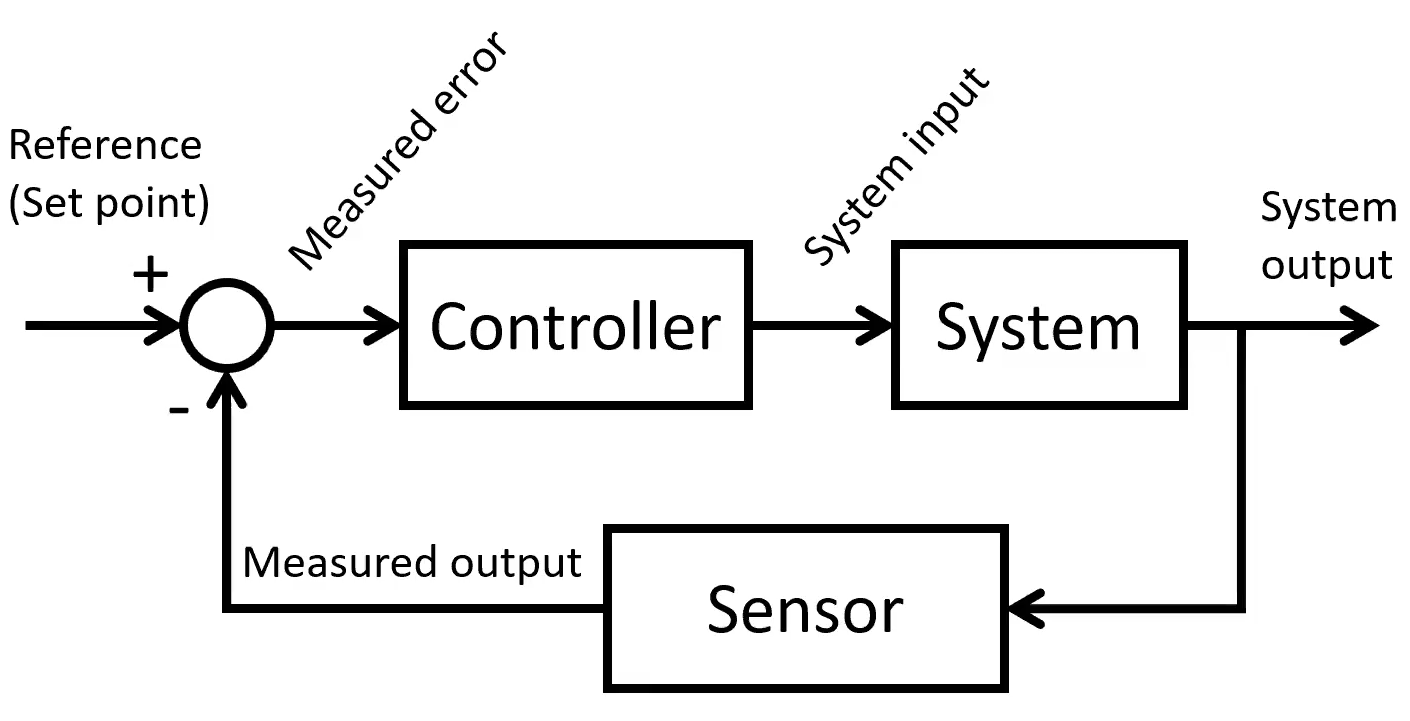
\includegraphics[width=0.8\textwidth]{negFeedbackCtrlLoop}
    \caption{Negative feedback control loop flow diagram}
    \label{fig:negFeedbackCtrlLoop}
\end{figure}
\begin{figure}[h]
    \centering
    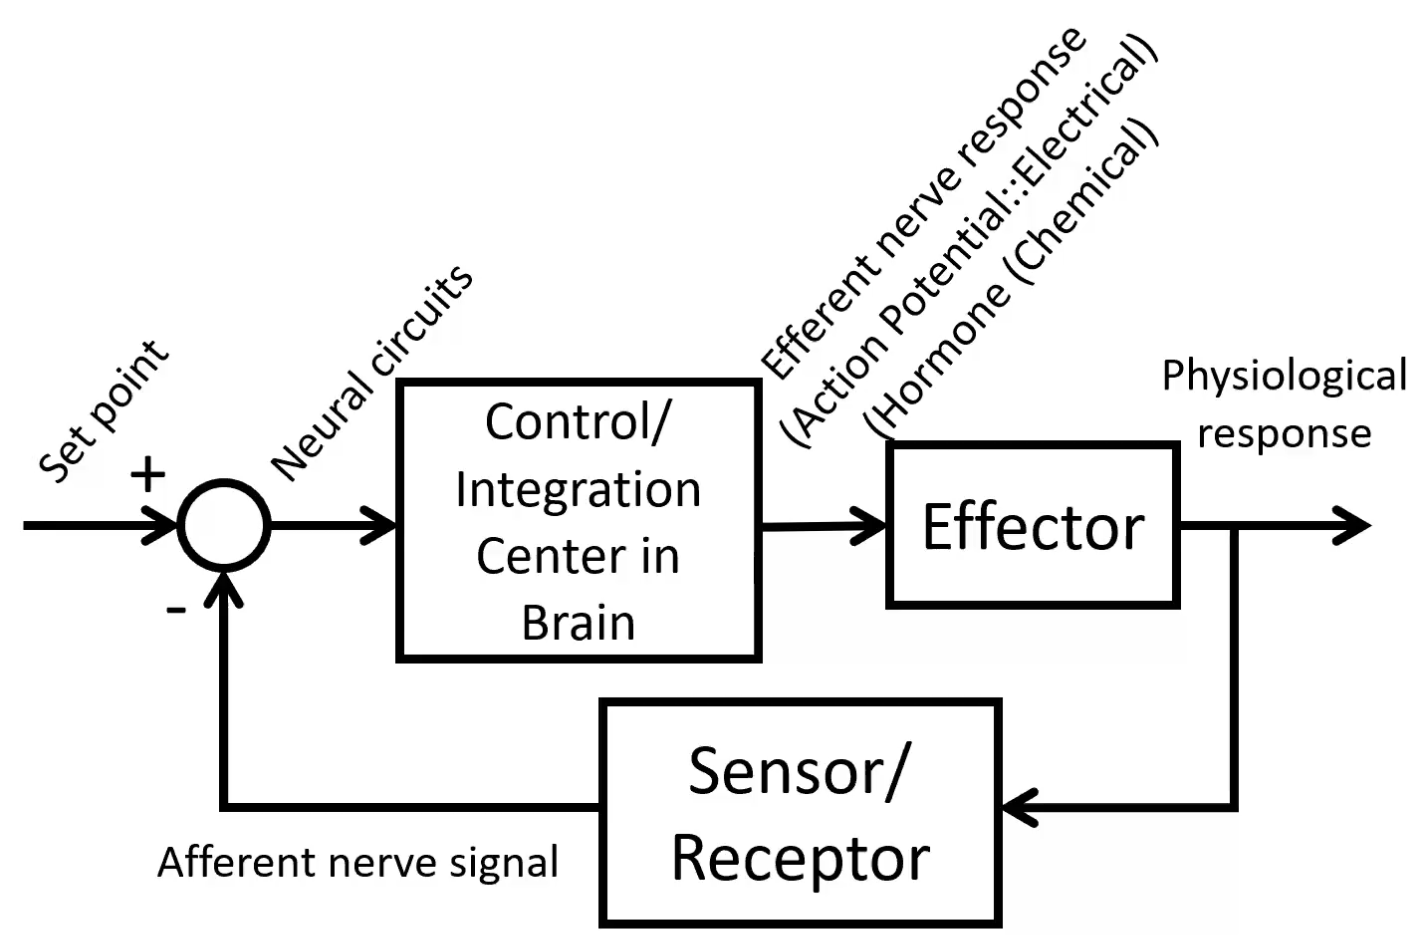
\includegraphics[width=0.8\textwidth]{negFeedbackCtrlLoopPhysioTerms}
    \caption{Same control loop but with more physiological terms}
    \label{fig:negFeedbackCtrlLoopPhysioTerms}
\end{figure}
\begin{itemize}
    \item idea is that the negative feedback is equivalent to some difference between a reference point $R$ and some sensor value $S$ :
\end{itemize}
\begin{figure}[h]
    \centering
    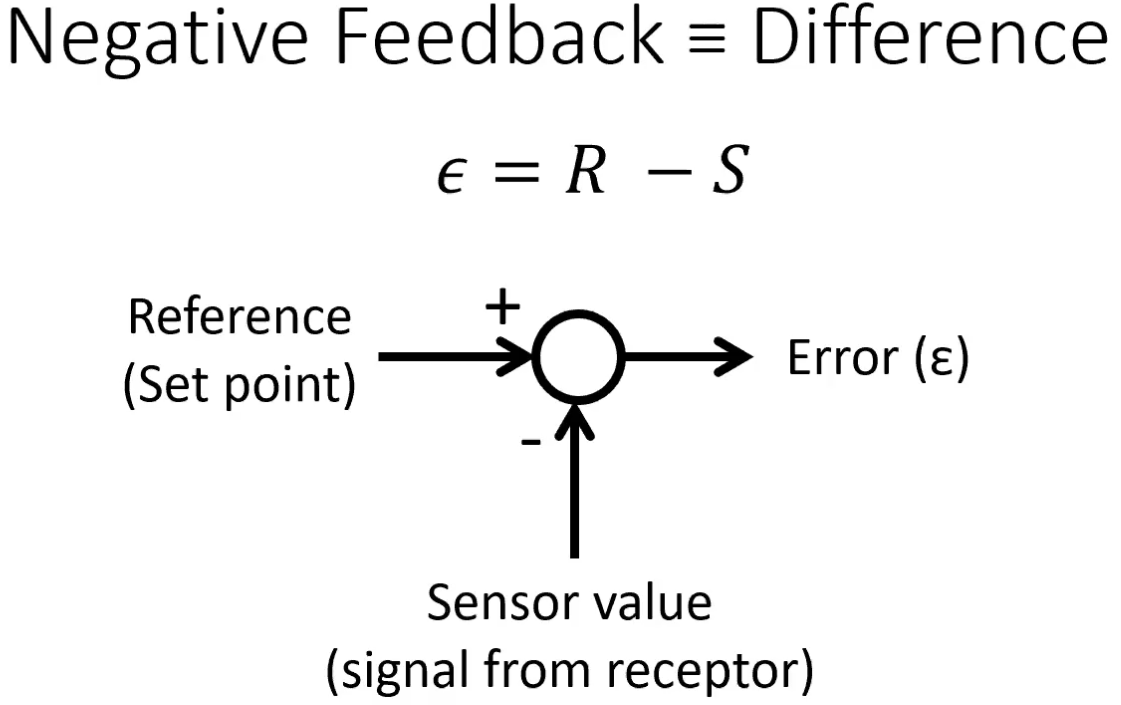
\includegraphics[width=0.7\textwidth]{negFeedbackIsDifference}
    \caption{}
    \label{fig:negFeedbackIsDifference}
\end{figure}
\begin{itemize}
    \item example: regulating body temperature
\end{itemize}
\begin{figure}[h]
    \centering
    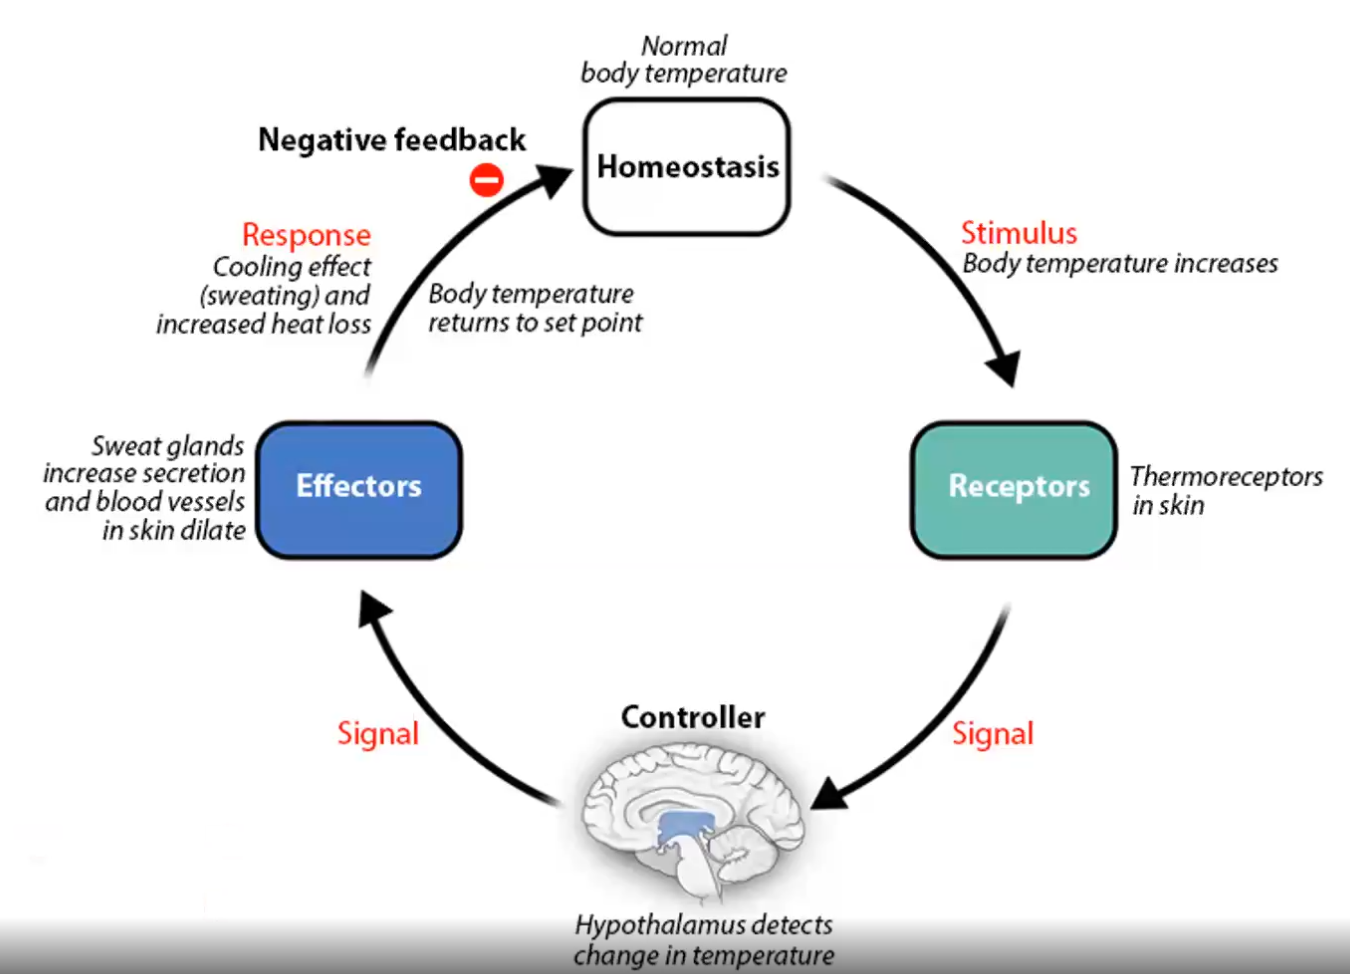
\includegraphics[width=0.8\textwidth]{regulateBodyTemperatureFeedbackLoop}
    \caption{}
    \label{fig:regulateBodyTemperatureFeedbackLoop}
\end{figure}
\begin{itemize}
    \item for any feedback loop, you should be able to identify:
    \begin{itemize}
        \item the physiological variable
        \item what and where the sensor is 
        \item where in the brain the control centre is 
        \item what and where the effectors are
    \end{itemize}
\end{itemize}



\part{Cell Physiology}

\section{Cell Structure}
\begin{figure}[h]
    \centering
    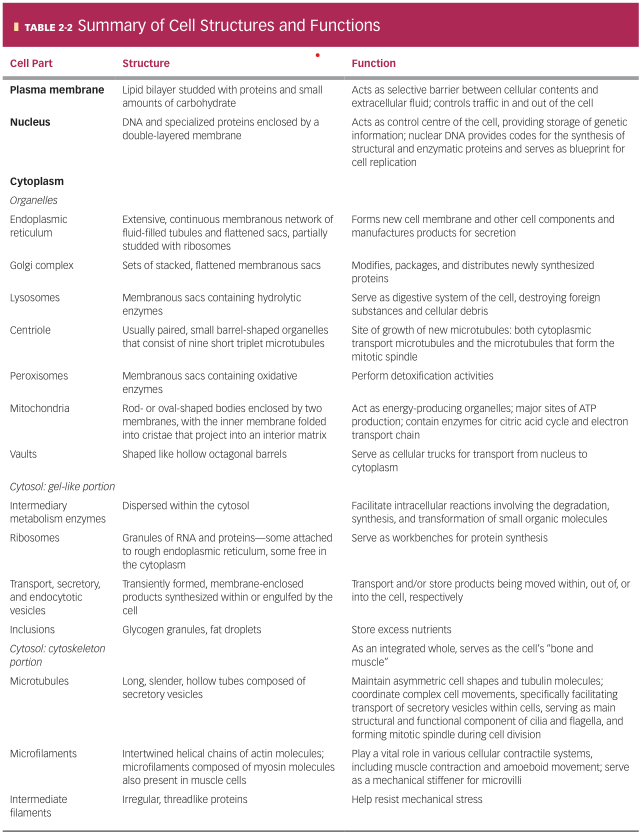
\includegraphics[width=0.9\textwidth]{cellStructuresAndFunctions}
    \caption{Cell Structures and Functions}
    \label{fig:Cell Structures and Functions}
\end{figure}
\begin{figure}[h]
    \centering
    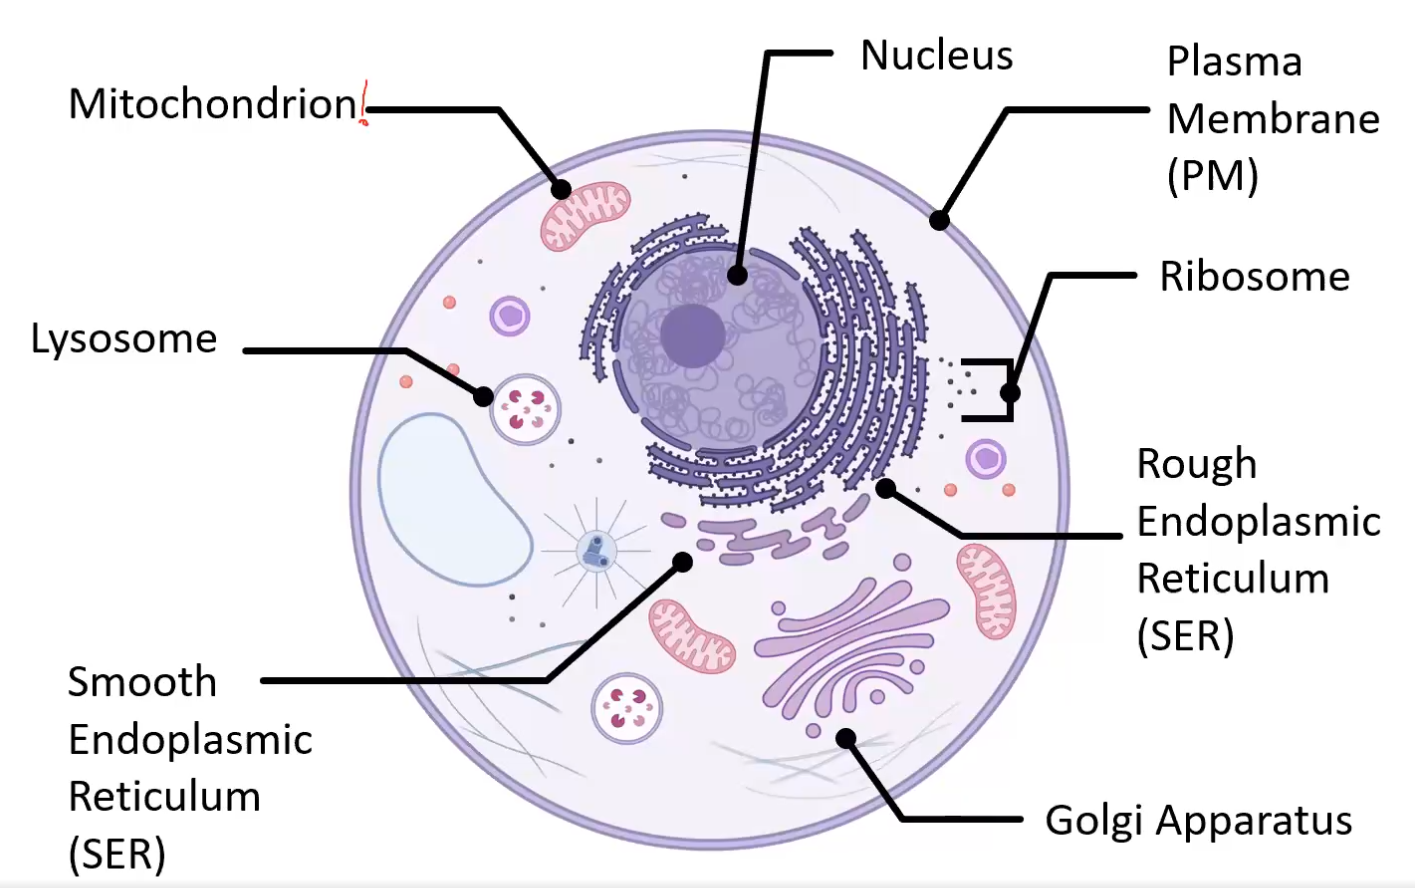
\includegraphics[width=0.6\textwidth]{cellOrganelles}
    \caption{Cell organelles.}
    \label{fig:cellOrganelles}
\end{figure}
\subsubsection{The Nucleus}
\begin{itemize}
    \item control centre of cell
    \item has a nuclear envelope made of two lipid bilayer membranes
    \item passageways for proteins, called "pores"
    \item inside nucleus: the nucleolus, responsible for manufacturing RNA (necessary for construction of ribosomes)
    \begin{figure}[h]
        \centering
        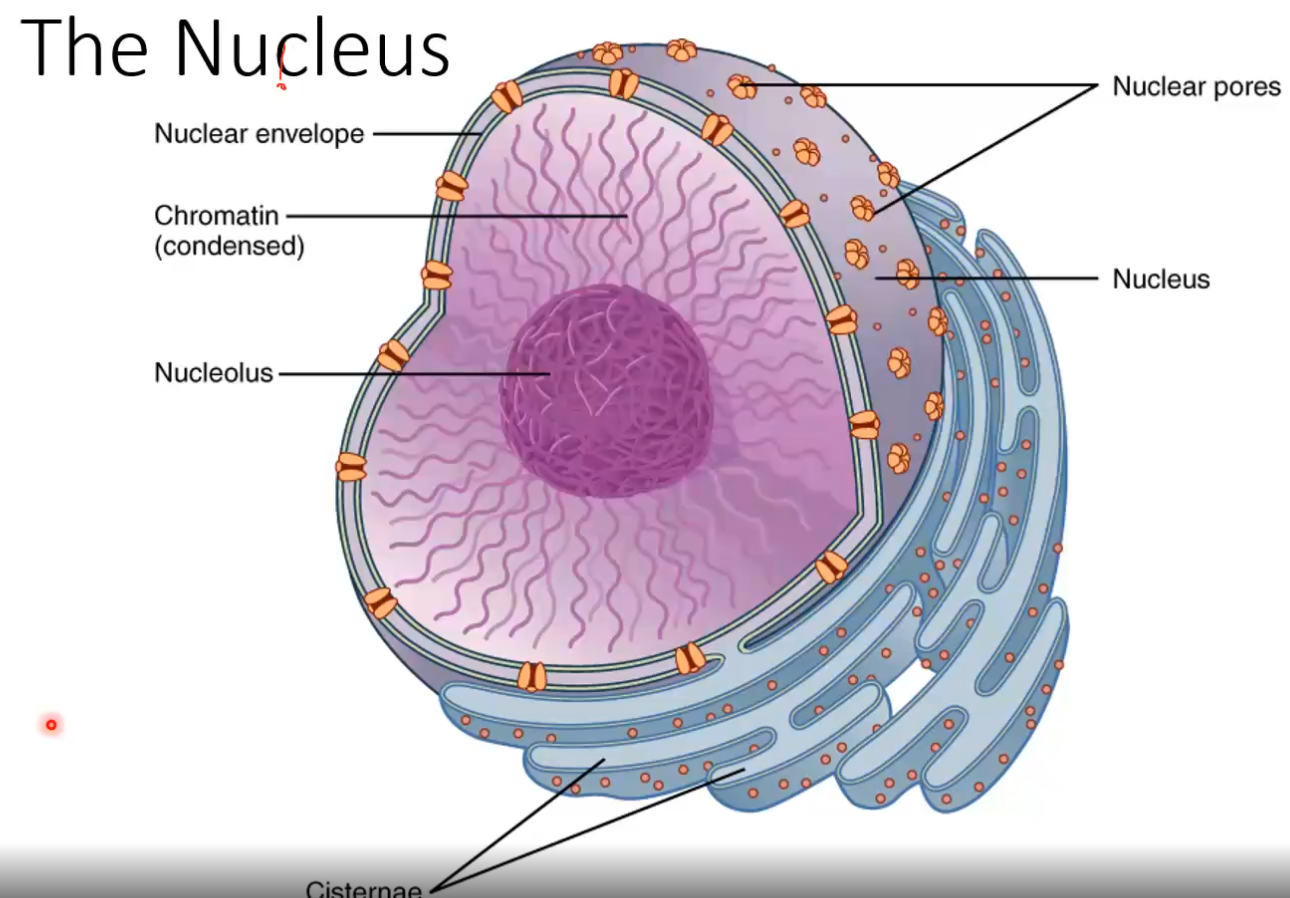
\includegraphics[width=0.6\textwidth]{nucleus}
        \caption{The nucleus.}
        \label{fig:nucleus}
    \end{figure}
\end{itemize}

\section{DNA Transcription and Translation}
\begin{itemize}
    \item DNA -- double stranded nucleic acid that stores genetic information
\subsection{DNA Structure}
    \item made from 2 polynucleotide chains
    \item DNA supercoils into chromosomes
    \item Levels of complexity of DNA are shown in Figure \ref{fig:DNA}
\begin{figure}[h]
    \centering
    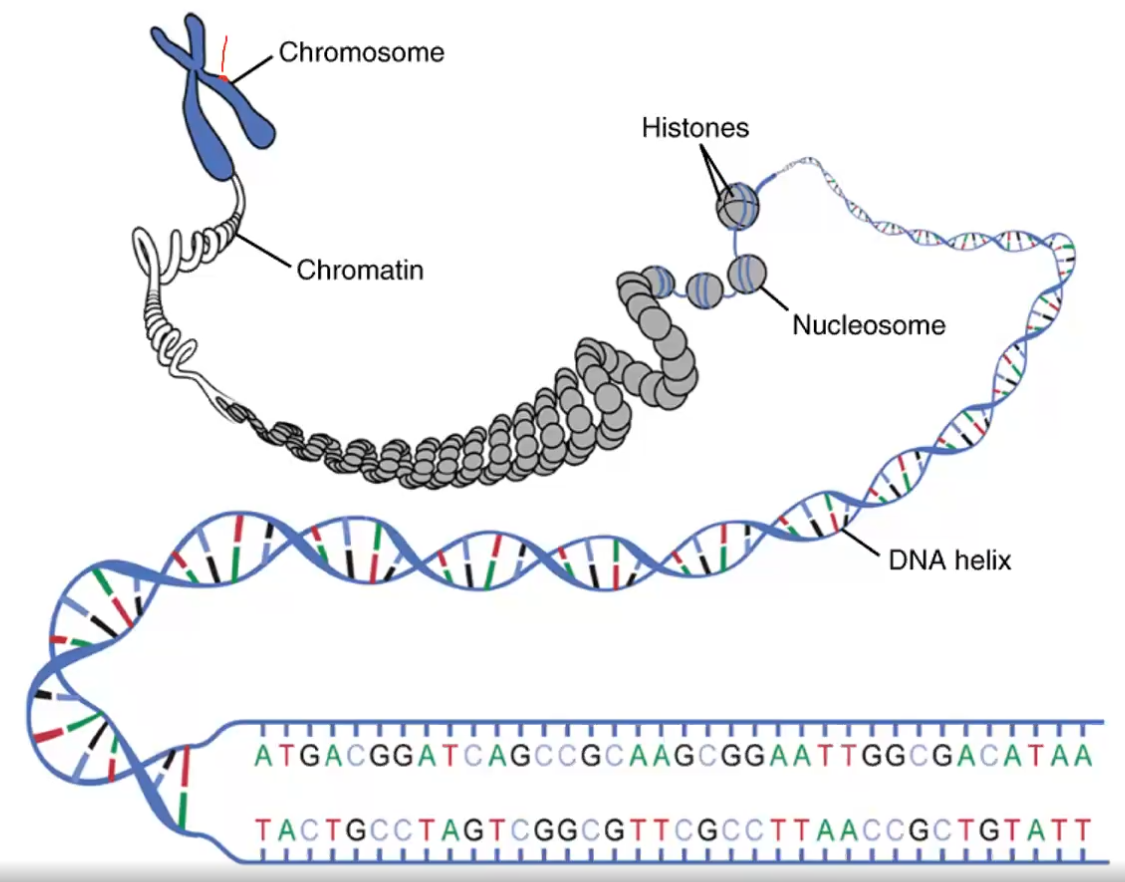
\includegraphics[width=0.8\textwidth]{DNA}
    \caption{Levels of complexity of DNA.}
    \label{fig:DNA}
\end{figure}
\begin{figure}[h]
    \centering
    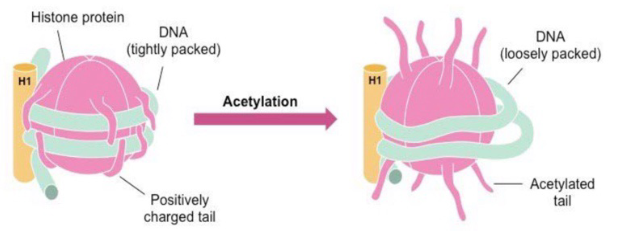
\includegraphics[width=0.8\textwidth]{histoneTails}
    \caption{Histone tails trap down the DNA.}
    \label{fig:histoneTails}
\end{figure}
\item there are different kinds of nucleosome packing: euchromatin for high transcriptional activity, heterochromatin for little to no transcriptional activity
\begin{figure}[h]
    \centering
    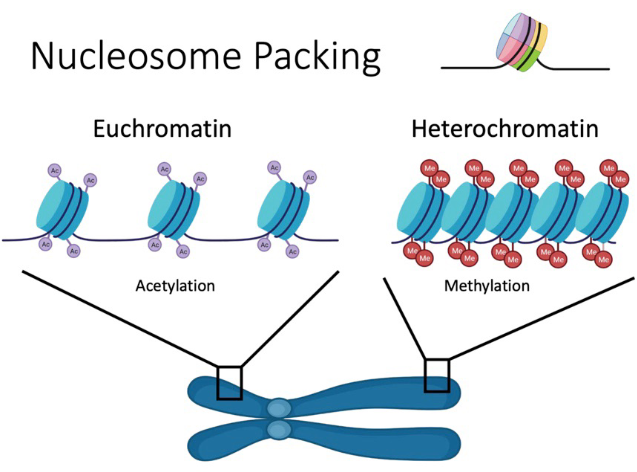
\includegraphics[width=0.8\textwidth]{nucleosomePacking}
    \caption{Nucleosome packing.}
    \label{fig:nucleosomePacking}
\end{figure}
\item each nucleotide contains a sugar (deoxyribose), phosphate group, and nitrogenous base
\item 4 N-bases: adenine (A), guanine (g), thymine (T), cytosine (C)
    \begin{itemize}
        \item C and T have one ring structure, G and A have two ring structure
    \end{itemize}
\item A-T pair, G-C pair
    \begin{figure}[h]
        \centering
        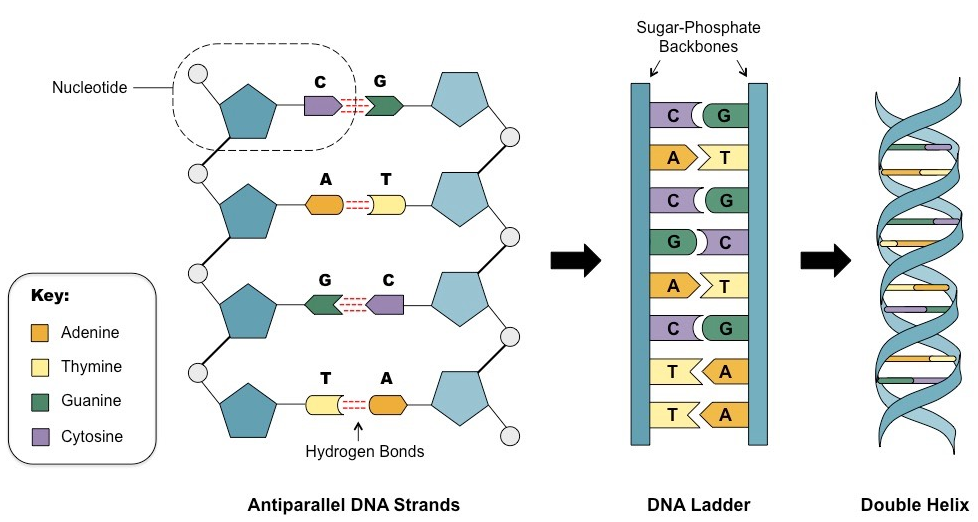
\includegraphics[width=0.8\textwidth]{DNAStructure}
        \caption{DNA structure.}
        \label{fig:DNAStructure}
    \end{figure}
\end{itemize}

\subsection{DNA Transcription}
\begin{itemize}
    \item first step in gene expression: copy gene's DNA sequence to make an RNA molecule
    \item DNA is used as a template for complementary base-pairing
    \item performed by enzymes called RNA polymerase -- links nucleotides to form an RNA strand using DNA strand as template
    \item in eukaryotes, RNA must be processed after transcription (spliced and have 5' cap at beginning and 3' poly A tail)
\end{itemize}

\subsection{DNA Translation}
\begin{itemize}
    \item DNA translation has 3 stages: initiation, elongation, termination
    \item Initiation: ribosome joins mRNA and first tRNA to form initiation complex
    \item Elongation: amino acids are brought by tRNA and linked to form chain 
        \begin{itemize}
            \item protein chain gets longer 
        \end{itemize}
    \item Termination: finished protein is released to do job in cell 
        \begin{itemize}
            \item when 'stop' codon in mRNA (UAA, UAG, or UGA) enters A site, recognized by release factors (proteins)
            \item H$_2$O is added to the acid, causing separation
        \end{itemize}
        \begin{figure}[h]
            \centering
            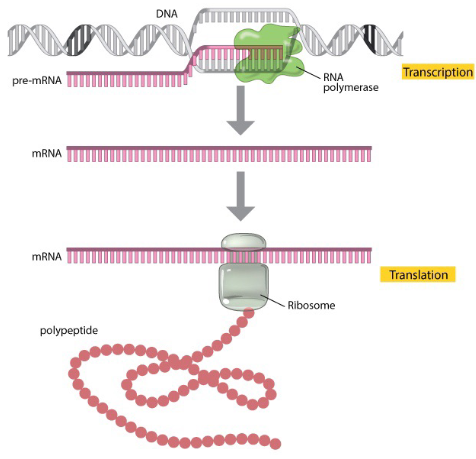
\includegraphics[width=0.8\textwidth]{DNATranscriptionTranslation}
            \caption{Summary of DNA transcription and translation.}
            \label{fig:DNATranscriptionTranslation}
        \end{figure}
\end{itemize}



\section{Cellular Metabolism}
\begin{itemize}
    \item \textbf{intermediary metabolism}: chemical reactions inside the cell that involve degradation, synthesis, and transformation of small organic molecules (e.g. sugars, amino acids, and fatty acids)
        \begin{itemize}
            \item all of these chemical reactions happen in the cytoplasm
            \item most of it happens in the cytosol, which contains thousands of enzymes involved in glycolysis and other intermediary biochemical reactions
        \end{itemize}
    \item \textbf{Anabolic processes}: synthesis of molecules for building up organs and tissues
    \item \textbf{Catabolic processes}: breakdown of complex molecules into simple ones
    \item cells require energy for anabolic processes (building complex molecules)
    \item this energy comes from carbon bonds of ingested food
    \item cells convert this energy into a usable form of energy: high-energy phosphate bonds in \textbf{adenosine triphosphate (ATP)}
    \item to obtain energy from ATP, cells split phosphate bond in ATP, which gives \textbf{adenosine diphosphate (ADP)}:
        \begin{align*}
            \text{ATP $\to$ ADP + $P_i$ + energy for use by the cell}
        .\end{align*}
    \item chemical pathways for production of ATP involve 3 separate processes:
        \begin{enumerate}
            \item substrate-level phosphorylation
            \item anaerobic glycolysis
            \item aerobic metabolism
        \end{enumerate}
    \item majority of ATP is generated from sequential dismantling of absorbed nutrient molecules in 4 steps:
        \begin{enumerate}
            \item glycolysis (both aerobic and anaerobic)
            \item decarboxylation of pyruvate
            \item tricarboxylic acid cycle (TCA; aerobic)
            \item electron transport chain (ETC; aerobic)
        \end{enumerate}
        \begin{figure}[h]
            \centering
            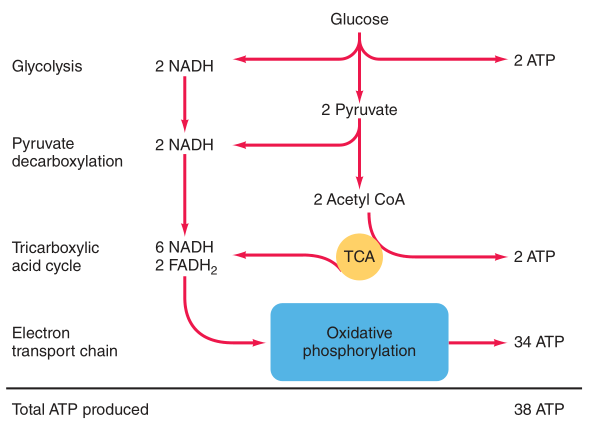
\includegraphics[width=0.7\textwidth]{ATPProductionOverview}
            \caption{Overview of ATP production. Maximum theoretical yield from 1 glucose is 38 ATP.}
            \label{fig:ATPProductionOverview}
        \end{figure}
\end{itemize}

\subsubsection{Pathways for Production of ATP}
\subsubsection*{Substrate-Level Phosphorylation}
\begin{itemize}
    \item some tissues (skeletal muscle) have low concentrations of ATP -- need to have quick ready supply of ATP
    \item \textbf{phosphorylation}: adding phosphate group to an organic molecule
    \item phosphorylation of ADP using creatine phosphate (CP) generates ATP
    \item reaction catalyzed by skeletal muscle cell enzyme creatine kinase
        \begin{align*}
            \text{CP + ADP $\longleftrightarrow$ creatine + ATP}
        .\end{align*}
\end{itemize}

\subsubsection*{Glycolysis}
\begin{itemize}
    \item breaks down glucose into 2 pyruvic acid molecules
    \item occurs in the cytosol
    \item some of the released energy is directly used to convert ADP to ATP while also producing NADH
    \item not really efficient at it though: most of the energy is still stored in the pyruvic acid molecules produced (what the mitochondria is for)
        \begin{figure}[h]
            \centering
            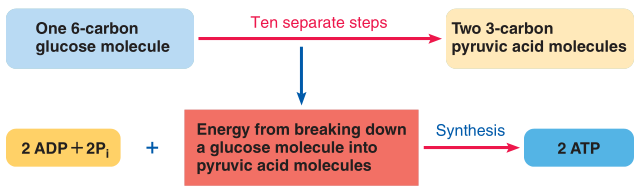
\includegraphics[width=0.8\textwidth]{glycolysis}
            \caption{Simplified summary of glycolysis. Net yield of 2 ATP and 2 NADH.}
            \label{fig:glycolysis}
        \end{figure}
\end{itemize}

\subsubsection*{Pyruvate Decarboxylation}
\begin{itemize}
    \item pyruvic acid (produced in cytosol by glycolysis) enters mitochondrial matrix through carrier protein monoccarboxylate transporter (located on inner mitochondrial membrane)
    \item inside mitochondria: pyruvate is metabolized by pyruvate dehydrogenase complex and decarboxylated
        \begin{itemize}
            \item Decarboxylation: removal of a carbon, formation of CO$_2$, and formation of 1 NADH
        \end{itemize}
    \item pyruvate is converted to acteyl CoA -- now ready to enter TCA cycle
\end{itemize}

\subsubsection*{Tricarboxylic Acid Cycle}
\begin{itemize}
    \item key purpose of Krebs cycle: produce hydrogens for entry into the ETC, which will be caught by NAD$^+$ and FAD to form NADH and FADH$_2$
    \item the 2 carbons from acetyl CoA are converted into CO$_2$
    \item oxaloacetic acid accepts acetyl CoA at start of cycle, and is regenerated at the end of cycle for use again
    \item 1 molecule of ATP is produced for each acetyl CoA
        \begin{figure}[h]
            \centering
            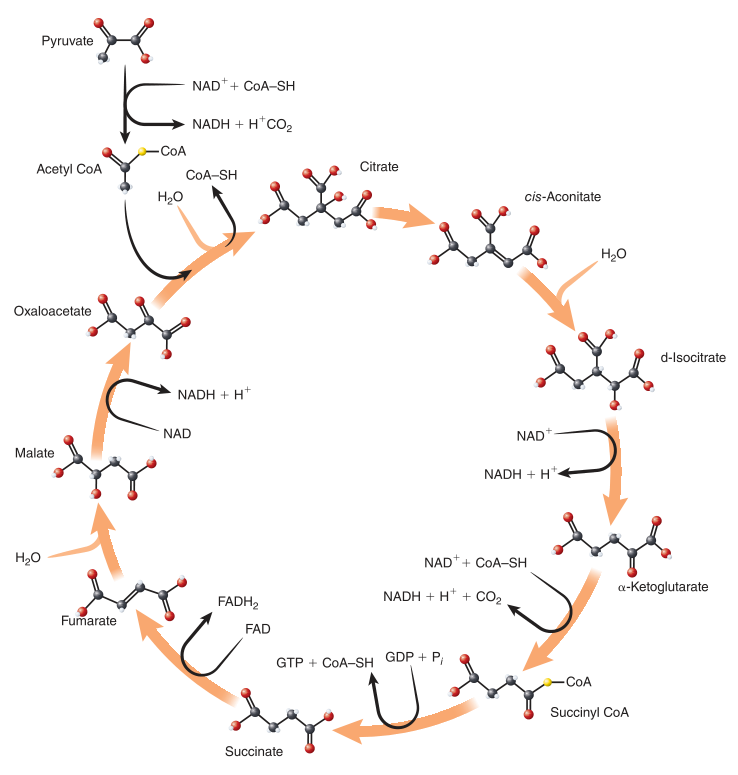
\includegraphics[width=0.6\textwidth]{krebsCycle}
            \caption{Krebs Cycle. }
            \label{fig:krebsCycle}
        \end{figure}
\end{itemize}

\subsubsection*{Electron Transport Chain}
\begin{itemize}
    \item NADH and FADH$_2$ drop off hydrogens at ETC
    \item hydrogen ions are pumped into intermembrane space -- build up high concentration
    \item the enzyme ATP synthase is activated by the flow of hydrogen ions back to the mitochondrial matrix and makes ATP through oxidative phosphorylation
    \item NADH enters ETC early, produces 3 ATP; FADH$_2$ enters later, produces 2 ATP
        \begin{figure}[h]
            \centering
            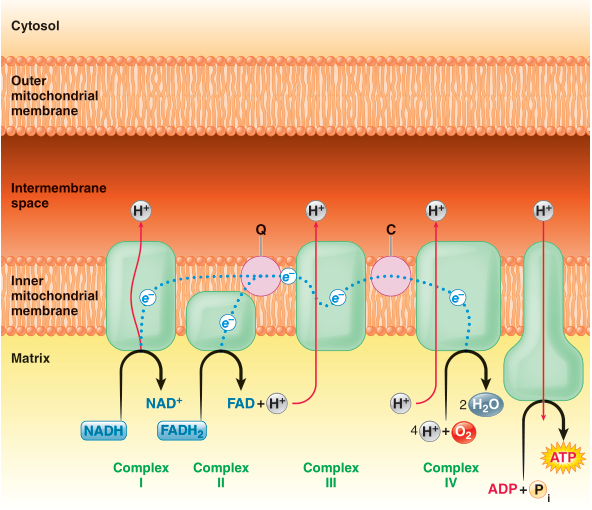
\includegraphics[width=0.6\textwidth]{ETC}
            \caption{Oxidative phosphorylation at the Electron Transport Chain. ATP synthesis relies on movement of hydrogen ions across inner mitochondrial membrane.}
            \label{fig:ETC}
        \end{figure}
\end{itemize}

\subsubsection{Practical ATP Yield}
\begin{itemize}
    \item theoretical maximum of 38 ATP assumes: (1) NADH produced in glycolysis in the cytosol doesn't need energy to be transported to the ETC, (2) ETC is 100\% efficient
        \begin{itemize}
            \item cells may require ATP to shuttle NADH from cytosol into mitochondria
            \item ETC usually produces 2 or 3 ATP from NADH (use 2.5) and 1 or 2 from FADH$_2$ (use 1.5)
        \end{itemize}
    \item actual yield is around 30 to 32 ATP (depending on how NADH from glycolysis gets to the ETC)
\end{itemize}


\section{The Cell Membrane}
\begin{itemize}
    \item bounds cells
    \item thin lipid bilayer with interspersed proteins with carbohydrates on outer surface
    \item cholesterol is tucked in the layer and helps with fluidity and stability of membrane
    \item bilayer is embedded with proteins with many purposes:
        \begin{itemize}
            \item channels for passage of small ions across teh membrane 
            \item carriers for transport of specific substances in or out of the cell 
            \item docking-marker acceptors for fusion with and subsequent exocytosis of secretory vesicles ????????
            \item membrane-bound enzymes that govern specific chemical reactions 
            \item receptors for detecting and responding to chemical messengers that alter cell function 
            \item cell adhesion molecules that help hold cells together and serve as a structural link between the extracellular surroundings and intracellular cytoskeleton
        \end{itemize}
    \item membrane carbohydrates serve as self-identity markers -- important for cell to cell interactions
        \begin{figure}[h]
            \centering
            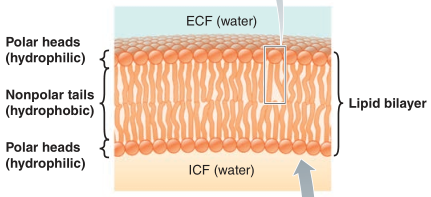
\includegraphics[width=0.6\textwidth]{phospholipidBilayer}
            \caption{Phospholipid bilayer.}
            \label{fig:phospholipidBilayer}
        \end{figure}
        \begin{figure}[h]
            \centering
            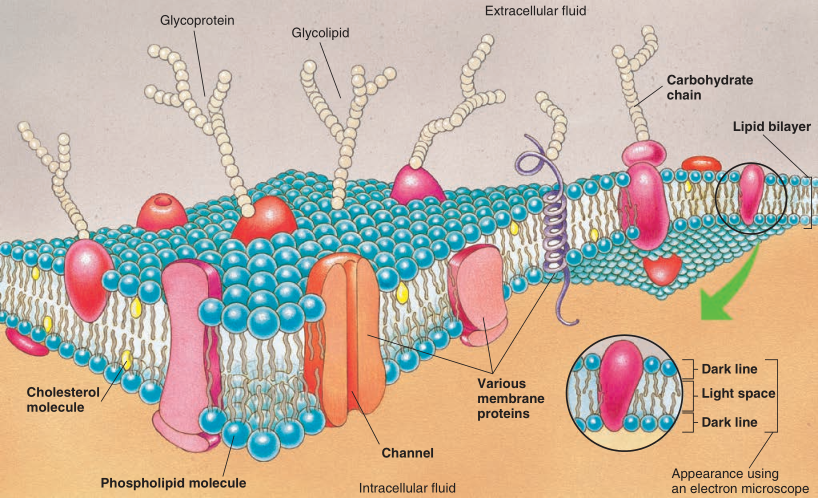
\includegraphics[width=0.8\textwidth]{plasmaMembraneStructure}
            \caption{Fluid mosaic model of plasma membrane structure.}
            \label{fig:plasmaMembraneStructure}
        \end{figure}
\end{itemize}


\section{Cell-to-Cell Adhesions}
\begin{itemize}
    \item some cells need to stay together (cells of the same tissue)
    \item some cells within given types of tissues are directly linked by gap junctions (specialized cell junction)
\end{itemize}
\subsection{Gap Junctions}
\begin{itemize}
    \item communicating junctions between 2 adjacent, but not touching cells 
    \item connected by small tunnels made up of connexons that permit exchange of ions and small molecules between adjacent cells 
    \item important in spreading electrical activity
        \begin{figure}[h]
            \centering
            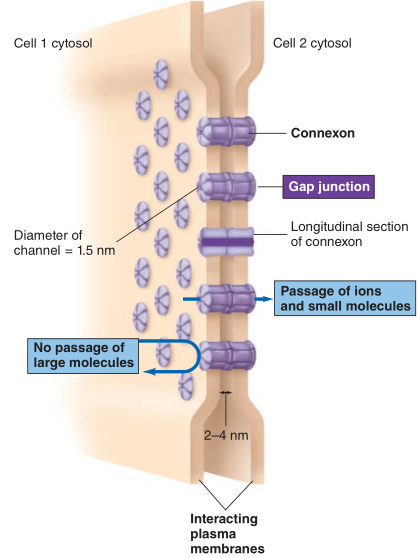
\includegraphics[width=0.4\textwidth]{gapJunction}
            \caption{Gap junction.}
            \label{fig:gapJunction}
        \end{figure}
\end{itemize}


\section{Membrane Transport}
\begin{itemize}
    \item materials can be passed between extracellular fluid (ECF) and intracellular fluid (ICF) by unassisted/assisted means
    \item transport mechanisms can be: 
        \begin{itemize}
            \item passive -- particle moves across membrane without cell expending energy
            \item active -- cell must expend energy
        \end{itemize}
\end{itemize}


\section{Unassisted Membrane Transport}
\begin{itemize}
    \item for lipid-soluble particles/ions
    \item \textbf{Diffusion}: for non-polar (lipid soluble) moleuclues of any size can dissolve in and pass through bilayer down gradients
        \begin{itemize}
            \item small ions traverse membrane passively down electro-chemical gradients through specific open protein channels
        \end{itemize}
    \item \textbf{Osmosis} -- special case where water passively moves down its own concentration gradient to area with higher solute concentration
\end{itemize}


\section{Assisted Membrane Support}
\begin{itemize}
    \item for small polar molecules and selected ion movements
\end{itemize}
\subsection{Carrier-mediated transport}
\begin{itemize}
    \item particle transported by specific membrane carrier proteins
    \item carrier-mediated transport takes two forms: passive (facilitated diffusion) and active transport
    \item carriers can move:
        \begin{itemize}
            \item 1 substance in one direction
            \item 2 in opposite direction
            \item 2 in same direction
        \end{itemize}
\end{itemize}
\subsubsection{Passive transport}
\begin{itemize}
    \item facilitated diffusion down concentration gradient (high to low concentration)
        \begin{figure}[h]
            \centering
            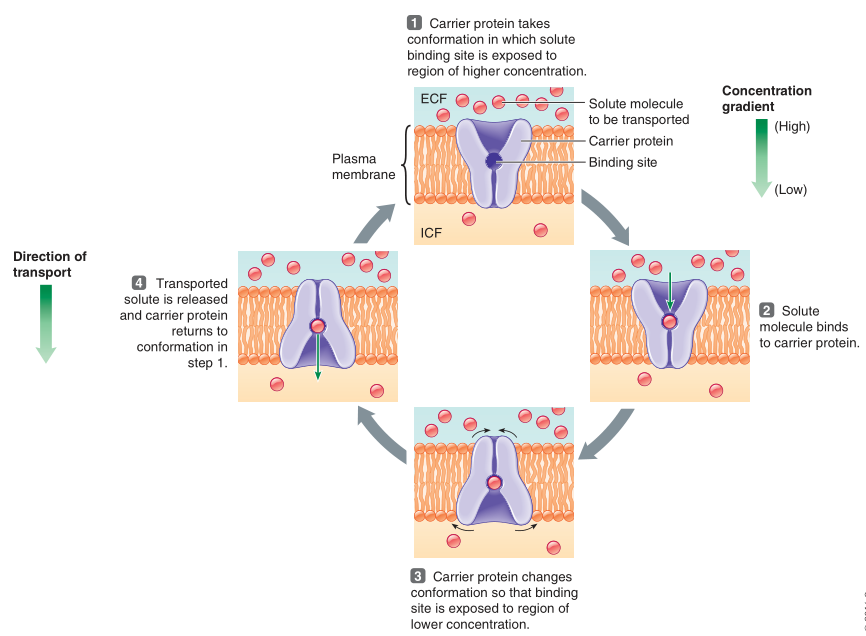
\includegraphics[width=0.8\textwidth]{facilitatedDiffusion}
            \caption{Example of facilitated diffusion.}
            \label{fig:facilitatedDiffusion}
        \end{figure}
        \begin{figure}[h]
            \centering
            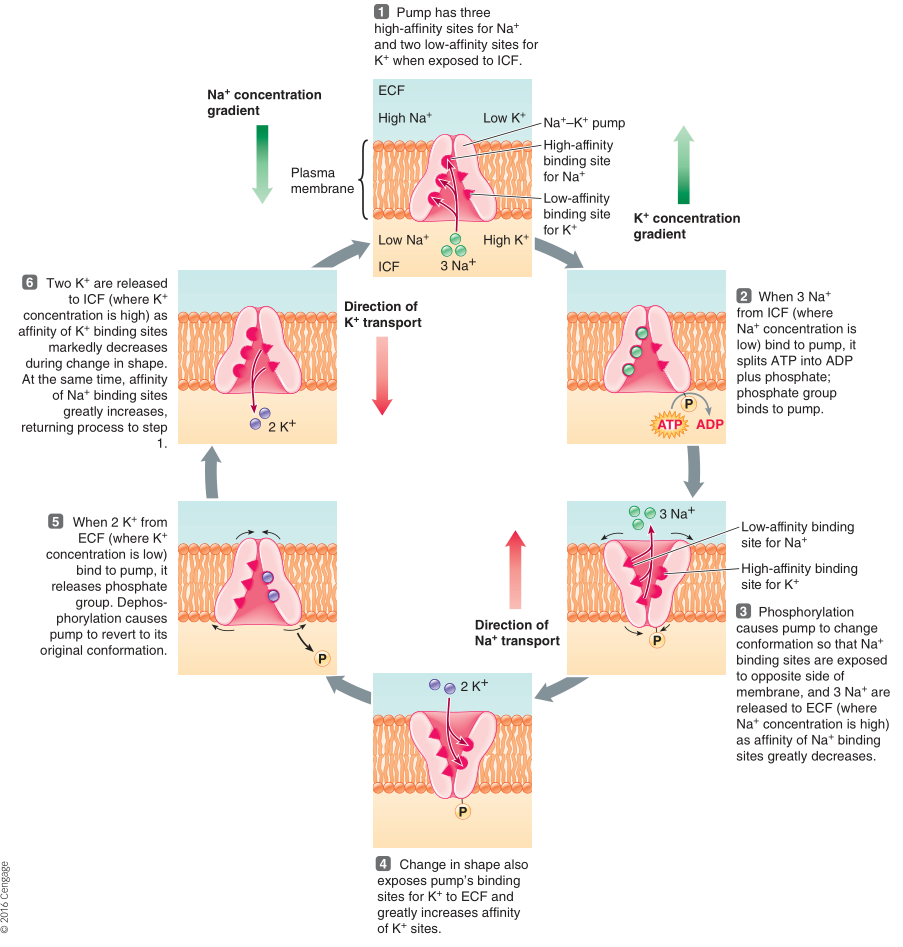
\includegraphics[width=0.8\textwidth]{NaKPump}
            \caption{Na$^+$-K$^+$ ATPase pump. Important example of primary active transport. It uses energy in the carrier's phosphorylation-dephosphorylation cycle to sequentially transport Na ion out of the cell and K ion into the cell against their concentration gradients. It moves 3 Na out and 2 K in for each ATP split.}
            \label{fig:NaKPump}
        \end{figure}
\end{itemize}
\subsubsection{Active transport}
\begin{itemize}
    \item requires carrier to expend energy to transfer particle against concentration gradient (low to high concentration)
\end{itemize}
\subsubsection*{Primary Active Transport}
\begin{itemize}
    \item requires ATP directly to drive the pump
\end{itemize}
\subsubsection*{Secondary Active Transport}
\begin{itemize}
    \item energy is not directly required to run the pump
    \item uses second-hand energy stored in the form of ion concentration gradient (e.g. Na$^+$ gradient) made by primary active transport
\end{itemize}

\subsection{Vesicular Transport}
\begin{itemize}
    \item for large polar molecules (since some can't permeate the membrane)
    \item leave (exocytosis) and enter (endocytosis) cell by being wrapped in a piece of membrane to form a vesicle
\end{itemize}

\begin{figure}[h]
    \centering
    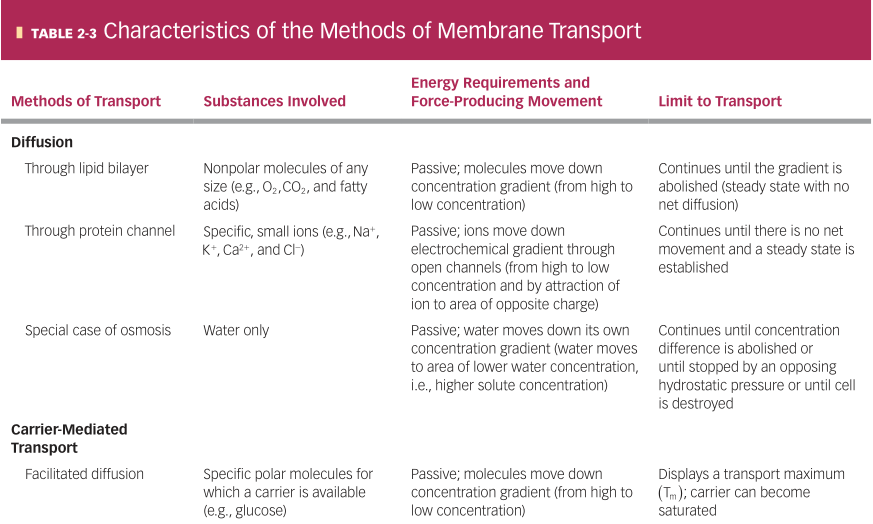
\includegraphics[width=0.8\textwidth]{membraneTransportMethods1}
    \caption{Table of membrane transport methods.}
    \label{fig:membraneTransportMethods1}
\end{figure}
\begin{figure}[h]
    \centering
    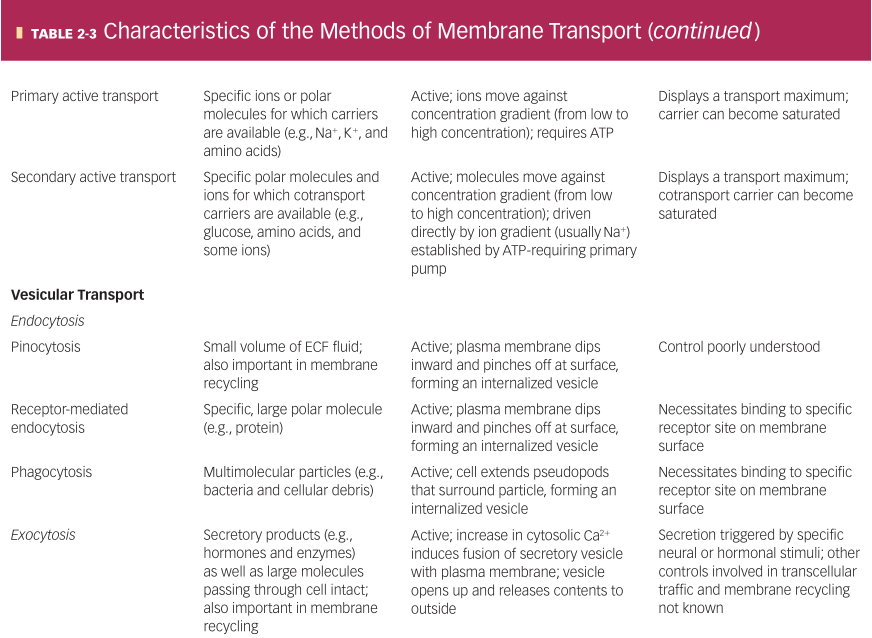
\includegraphics[width=0.8\textwidth]{membraneTransportMethods2}
    \caption{Table of membrane transport methods, continued.}
    \label{fig:membraneTransportMethods2}
\end{figure}


\section{Intracellular Communication}
\begin{itemize}
    \item cells need to communicate with each other to do stuff
\end{itemize}


\section{Membrane Potential}
\begin{itemize}
    \item separation of opposite charges due to relative number of cations and anions in the ICF vs ECF
    \item enables communication in nervous tissue and muscle
    \item \textbf{equilibrium potential}: the electric potential across the cell membrane when the electrical gradient exactly balances the concentration gradient of the ion
    \item equilibrium potential for a given ion of differing concentrations across a membrane is given by the \textbf{Nernst equation}:
        \begin{theorem}
            \textbf{Nernst Equation}: used to calculate equilibrium potential of an ion across a membrane
            \begin{align*}
                E_x = \frac{61}{Z_x} \log_{10} \frac{[C]_o}{[C]_i}
            \end{align*}
            \begin{itemize}
                \item $E_x$ -- equilibrium potential
                \item $Z_x$ -- valence (electrical charge for ion) (e.g. Z = 1 for Na ion)
                \item $[C]_o$ -- concentration outside cell
                \item $[C]_i$ -- concentration inside cell
            \end{itemize}
        \end{theorem}
\end{itemize}

\subsubsection*{Graphing Electrical-Chemical Gradients}
\begin{figure}[h]
    \centering
    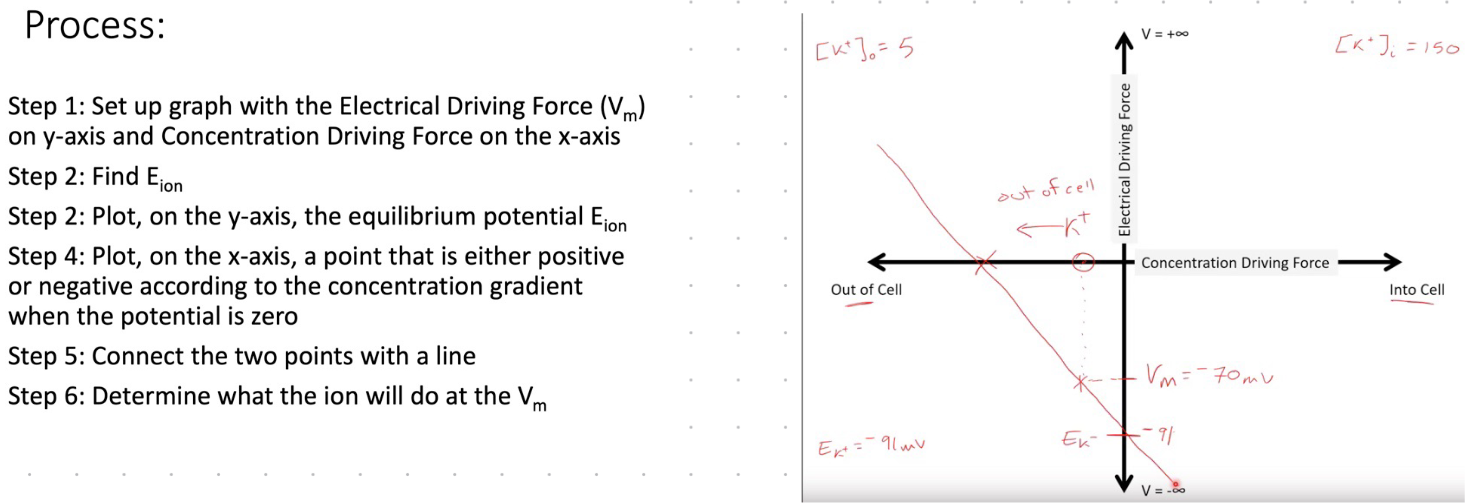
\includegraphics[width=0.8\textwidth]{graphingElecChemGradients}
    \caption{Process of grpahing electrical-chemical gradients.}
    \label{fig:graphingElecChemGradients}
\end{figure}

\subsubsection*{Equilibrium Potential Balances (Diffusion and Electrical Potential)}
\begin{gather*}
    \Delta G_{chem} = RT \ln \frac{[C]_o}{[C]_i} \\ 
    \text{and} \\ 
    \Delta G_{elec} = ZFV_m
.\end{gather*}
\begin{itemize}
    \item where $Z$ is charge, $F$ is Faraday's constant (96500), $V_m$ is voltage difference
    \item at equilibrium: $\Delta G_{chem} = \Delta G_{elec}$ 
    \item free energy moving out of cell:
        \begin{align*}
            \Delta G = \Delta G_{chem} - \Delta G_{elec}
        .\end{align*}
        \begin{itemize}
            \item if $\Delta G < 0$ : spontaneous (ion moves out of cell)
            \item if $\Delta G > 0$ : non-spontaneous (ion moves into cell)
        \end{itemize}
\end{itemize}



\section{Graded Potentials}
\begin{itemize}
    \item local changes in membrane potential that occur in varying grades or degrees of magnitude or strength
    \item may or may not lead to action potential
\end{itemize}

\section{Action Potentials}
\begin{itemize}
    \item brief, large, rapid changes in membrane potential -- potential reverses
    \item inside of excitable cell transiently becomes more positive than outside
\end{itemize}
\subsubsection*{Conduction via a Nerve Fibre}
\begin{itemize}
    \item \textbf{Contiguous conduction}: along unmyelinated axons 
    \item \textbf{Saltatory conduction}: myelinated axons
    \item myelin acts like electrical tape with little bits exposed between
    \item Factors impacting speed of propogation:
        \begin{itemize}
            \item amount of myelination
            \item axon diameter
            \item temperature
        \end{itemize}
\end{itemize}




\section{Synapses}
\begin{itemize}
    \item \textbf{axon} (nerve fibre): conducts action potentials in undiminished fashion from axon hillock to terminals
    \item \textbf{synapse} (neural junction): site of transmission of electrical nerve impulses between 2 nerve cells (neurons)
    \item \textbf{synaptic cleft}: small space between neurons
    \item \textbf{presynaptic neuron}: sends signal
    \item \textbf{postsynaptic neuron}: receives signal
    \item chemical signals (neurotransmitters) packaged in vesciles and sent over
        \begin{figure}[h]
            \centering
            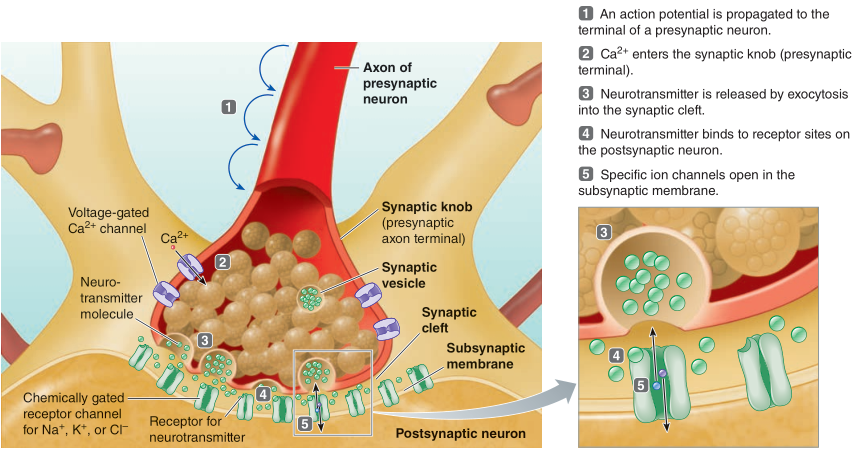
\includegraphics[width=0.8\textwidth]{synapticStructureAndFunction}
            \caption{Synaptic structure and function. The events that occur at a synapse.}
            \label{fig:}
        \end{figure}
\end{itemize}





\newpage
\part{The Central Nervous System}

\section{Organization of the Nervous System}
\begin{figure}[h]
    \centering
    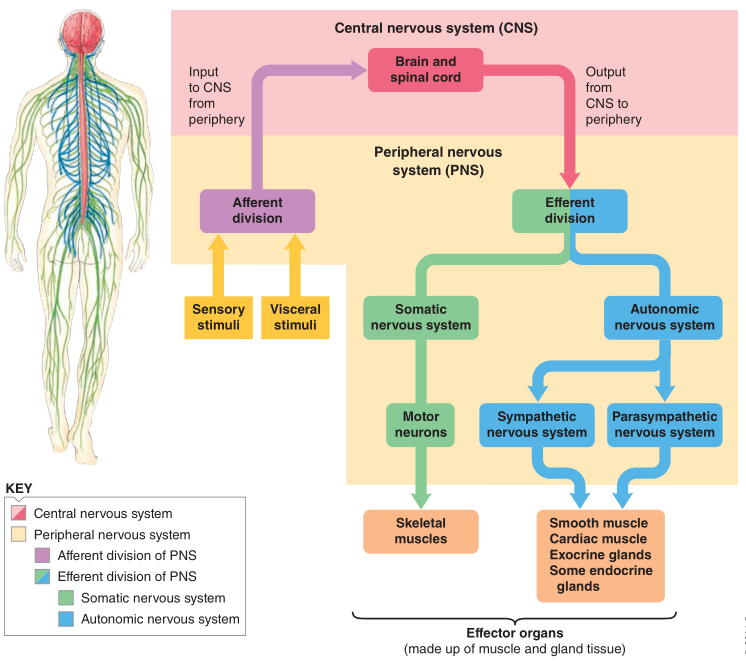
\includegraphics[width=0.8\textwidth]{nervousSystem}
    \caption{Organization of the Nervous System}
    \label{fig:nervousSystem}
\end{figure}
\begin{itemize}
    \item Central nervous system (CNS) consists of the brain and spinal cord 
    \item Peripheral nervous system (PNS) consists of fibres that carryinformation between the CNS and other body parts 
    \item the PNS is divided into the afferent and efferent divisions
    \item afferent -- carries information to the CNS 
    \item efferent -- carries signals from the CNS to the effector organs 
        \begin{itemize}
            \item 2 subdivisions in efferent division:
                \begin{enumerate}
                    \item Somatic nervous system: consists of nerve fibres of the motor neurons that control skeletal muscles (conscious control)
                    \item Autonomic nervous system consists of nerve fibres that innervate glands, cardiac muscles, and smooth muscles (unconscious control)
                        \begin{itemize}
                            \item further subdivided into sympathetic (for fight-or-flight) and parasympathetic (inhibits overworking) nervous system
                        \end{itemize}
                \end{enumerate}
        \end{itemize}
\end{itemize}

\subsection{Three Functional Classes of Neurons}
\begin{itemize}
    \item afferent, efferent, and interneurons
\end{itemize}
\subsubsection*{Afferent}
\begin{itemize}
    \item in the afferent division
    \item shaped differently from the other two
    \item has a sensory receptor at its peripheral ending 
        \begin{itemize}
            \item which generates action potentials in response to a stimulus (e.g. touch)
        \end{itemize}
    \item soma (cell body) is devoid of dendrites and adjacent to the spinal cord 
    \item peripheral axon (afferent fibre) extends from the receptor to the soma
    \item a short central axon passes from the soma to the spinal cord 
    \item action potentials go from receptor (distal end) to the spinal cord (proximal end)
\end{itemize}
\subsubsection*{Efferent}
\begin{itemize}
    \item receive signals from interneurons in the CNS and innervate its target
\end{itemize}
\subsubsection*{Interneurons}
\begin{itemize}
    \item connect signals from afferent to efferent
    \item makes up 99\% of neurons (100 billion)
    \item more complex actions require more interneurons between afferent and efferent
\end{itemize}
\begin{figure}[h]
    \centering
    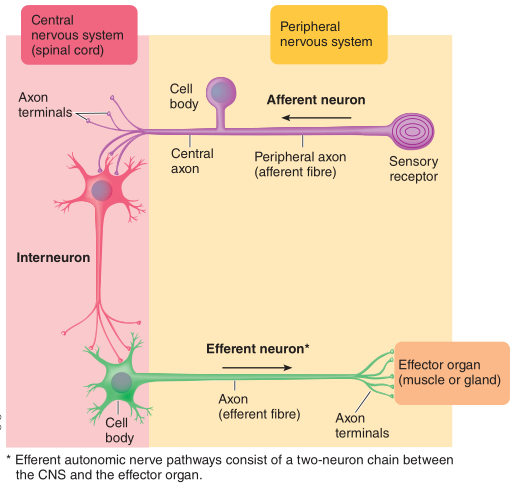
\includegraphics[width=0.8\textwidth]{threeClassesofNeurons}
    \caption{Organization and function of the three classes of neurons.}
    \label{fig:threeClassesofNeurons}
\end{figure}

\subsection{Glial Cells}
\begin{itemize}
    \item glial cells (or neuroglia) make up about 90\% of cells in the CNS 
    \item they don't initiate or conduct nerve impulses, but do communicate using chemical signals and maintain homeostasis
    \item serves as the connective tissue of the CNS
    \item maintains adequate extracellular composition for neuron activity
    \item modulates synaptic function, so they are considered nearly as important to memory as neurons
    \item 4 major types of glial cells: Astrocytes, Oligodendrocytes, Microglia, Ependymal cells
        \begin{itemize}
            \item astrocytes: induce formation of blook-brain barrier, take up exxcess K ions to maintain homeostasis, and degrade released neurotransmitters into raw materials for the synthesis of more neurotransmitters (most common too)
            \item oligodendrocytes: form myelin sheaths in CNS (in contrast to Schwann cells in PNS)
            \item microglia: play defense as phagocytic scavengers
            \item ependymal: line internal cavities of brain and spinal cord, contribute to cerebrospinal fluid formation and act as stem cells that can form new neurons and glial cells
        \end{itemize}
    \item learning occurs when myelin sheaths lengthen or new ones are created
        \begin{itemize}
            \item makes it more likely for APs to traverse the entire neuron 
            \item neuroplasticity -- neurons that fire together, wire together; neurons that fire out of sync, fail to link
        \end{itemize}
        \begin{figure}[h]
            \centering
            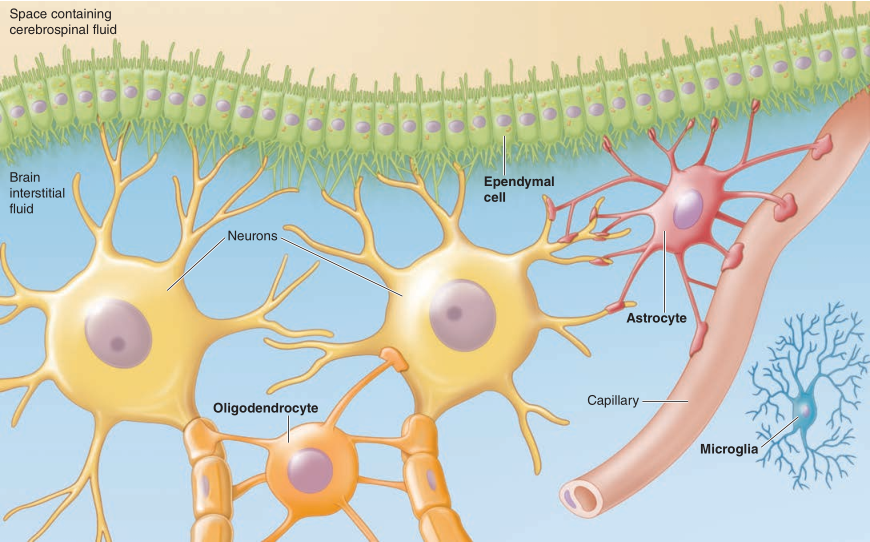
\includegraphics[width=0.8\textwidth]{glialCellsCNS}
            \caption{Glial cells of the central nervous system.}
            \label{fig:glialCellsCNS}
        \end{figure}
\end{itemize}


\subsection{Cerebrospinal Fluid}
\begin{itemize}
    \item has greater electrochemical gradient -- makes action potentials easier
\end{itemize}


\subsection{Anatomical Landmarks in the Brain and Spinal Cord}
\begin{itemize}
    \item cerebral cortex controls sensory perception, voluntary movement, personality, and sophisticated mental events like memory
    \item hypthalamus regulates temperature, thirst, urine output, food intake, and other homeostatic functions
        \begin{itemize}
            \item role in sleep-wake cycle 
            \item emotion and basic behaviour 
            \item important link between nervous and endocrine systems
        \end{itemize}
    \item cerebellum maintains balance and coordination 
    \item brainstem is control centre for cardiovascular, respiratory, and digestive systems
\end{itemize}

\subsection{Spinal Cord}
\begin{itemize}
    \item descends through vertical canal and is surrounded by the vertebral column
    \item spinal nerves are paired neurons that emerge from the spinal cord 
    \item from head to toe: 
        \begin{itemize}
            \item 8 cervical (neck) nerves
            \item 12 thoracic (chest) nerves
            \item 5 lumbar (abdominal) nerves
            \item 5 sacral (pelvic) nerves
            \item 1 coceygeal (tailbone) nerve
        \end{itemize}
        \begin{figure}[h]
            \centering
            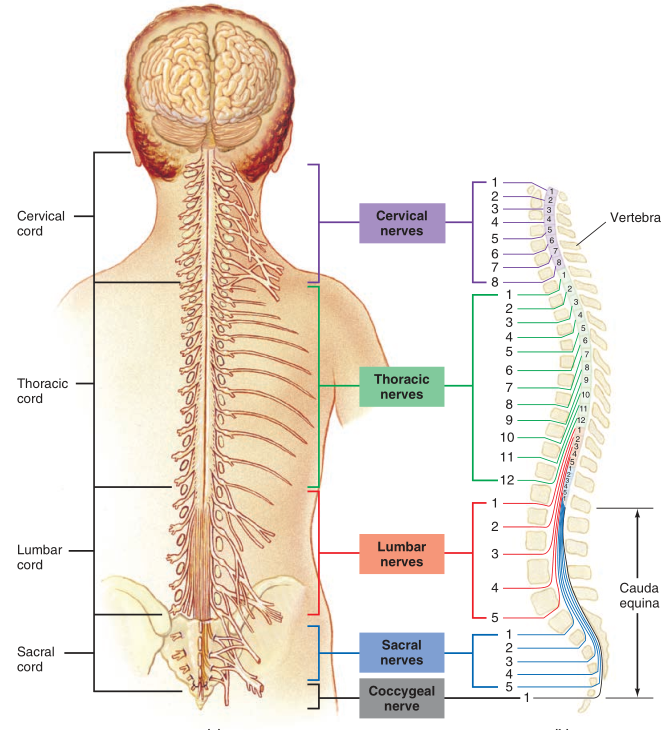
\includegraphics[width=0.8\textwidth]{spinalNerves}
            \caption{Spinal nerves.}
            \label{fig:spinalNerves}
        \end{figure}
\end{itemize}

\subsubsection{Spinal Cord in Cross-Section}
\begin{itemize}
    \item grey matter in spinal cord forms an inner butterfly-shaped region surrounded by white matter
    \item cord grey matter consists primarily of neuronal cell bodies and their dendrites, interneurons, and glial cells
    \item white matter consists primarily of myelinated neurons
        \begin{itemize}
            \item organized into tracts (bundles of nerve fibres/axons of long interneurons)
            \item ascending tracts go from cord to brain while descending tracts go brain to cord
        \end{itemize}
        \begin{figure}[h]
            \centering
            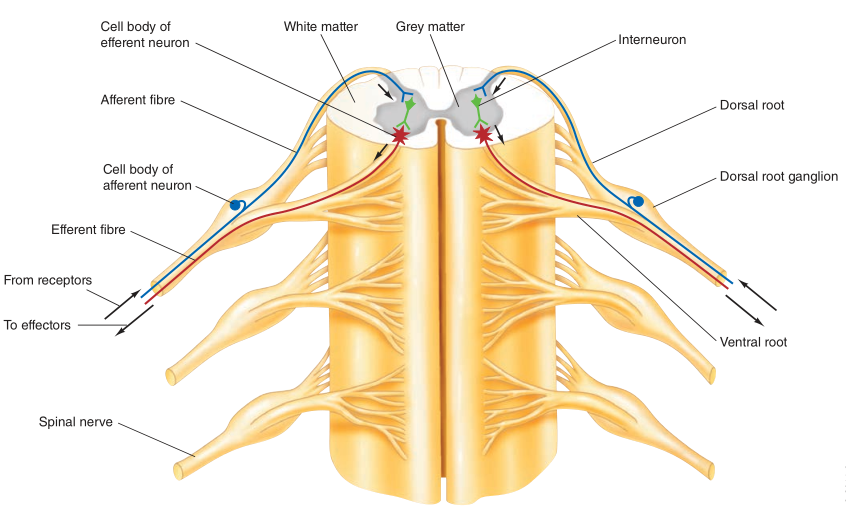
\includegraphics[width=0.8\textwidth]{spinalCordCrossSection}
            \caption{Spinal cord in cross section.}
            \label{fig:spinalCordCrossSection}
        \end{figure}
    \item sensory pathways have afferent neuron connect to an interneuron in the grey matter region, which then enters an ascending tract in the white matter region
        \begin{itemize}
            \item enters grey matter through dorsal root
        \end{itemize}
    \item motor neurons have interneuron travel down descending tract, goes from white matter to grey matter, connects to an efferent neuron, and exits out of the spinal cord through the ventral root
\end{itemize}


\subsection{Reflexes}
\begin{itemize}
    \item reflex: any response that occurs automatically without conscious effort
    \item nerve impulses that enter the spinal cord on the same side from which nerve impulses leave it are called reflex arcs
        \begin{itemize}
            \item a neural pathway that controls an action reflex
        \end{itemize}
    \item stretch reflex: involves an afferent neuron originating at a stretch-detecting receptor in a skeletal muscle (causing stretch)
        \begin{itemize}
            \item terminates on the efferent neuron innervating the same skeletal muscle
                \begin{itemize}
                    \item causes counteracting contraction
                    \item reciprocal innervation
                \end{itemize}
        \end{itemize}
    \item stretch reflex is caused by a reflex arc 
    \item stretch reflex is a mono-synaptic reflex (no interneurons) (e.g. knee jerk)
    \item polysynaptic reflexes have interneurons between the afferent and efferent neurons (e.g. withdrawal reflexes)
\end{itemize}


\subsection{Cranial Nerves}
\begin{itemize}
    \item most fibres pass through the brain stem 
    \item these include the 12 pairs of cranial nerves
        \begin{itemize}
            \item all but the vagus nerve of the cranial nerves supply structures in the head and neck with sensory and motor fibres
                \begin{itemize}
                    \item vagus nerve supplies organs in the thoratic and abdominal cavities
                    \item is the major nerve of the parasympathetic nervous system
                \end{itemize}
            \item includes glossopharyngeal nere -- controls the pharynx and hypoglosal nerve (which controls the tongue)
        \end{itemize}
\end{itemize}


\subsection{Cerebral Cortex}
\begin{itemize}
    \item the cerebrum is divided into left and right cerebral hemispheres
        \begin{itemize}
            \item connected by the corpus callosum
        \end{itemize}
    \item each hemisphere has a thin outer shell of grey matter (cerebral cortex) covering a thick core of white matter 
    \item grey matter acts like comuter and white matter acts like wires 
    \item 4 major lobes
        \begin{itemize}
            \item occipital, temporal, parietal, and frontal (back, side, middle top, front)
        \end{itemize}
    \item sensations from the body surface (touch, pressure, pain, etc.) are somaesthetic sensations
        \begin{itemize}
            \item information is projected to the somatosensory cortex (front of parietal lobe)
                \begin{itemize}
                    \item responsible for processing of somaesthetic and proprioceptive (awareness of body position) input
                    \item representation by body parts (to show what body parts are controlled where in the cortex) is the sensory homunculus
                        \begin{figure}[h]
                            \centering
                            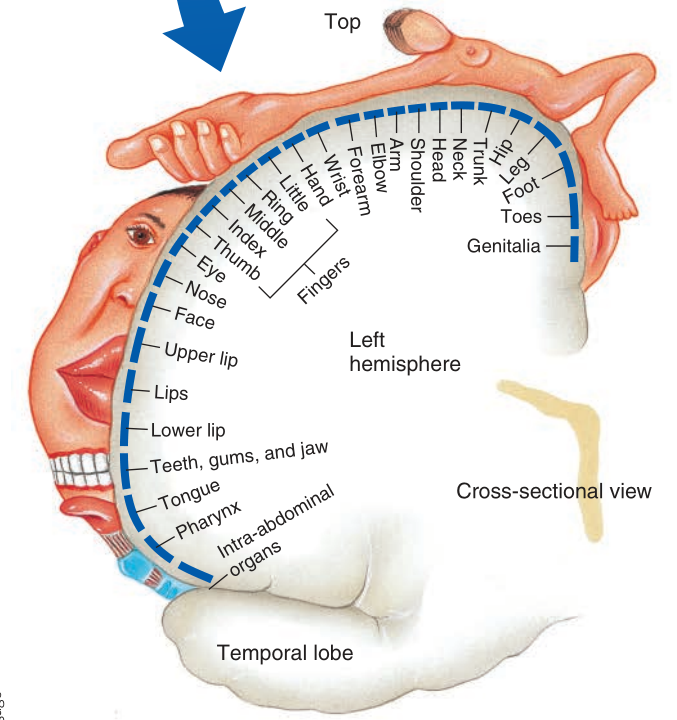
\includegraphics[width=0.8\textwidth]{sensoryHomunculus}
                            \caption{Sensory homunculus.}
                            \label{fig:sensoryHomunculus}
                        \end{figure}
                \end{itemize}
        \end{itemize}
    \item control of motor functions of skeletal muscles is done in the primary motor cortex 
        \begin{itemize}
            \item back of frontal lobe, in front of somatosensory cortex 
            \item representation by body parts is the motor homunculus
        \end{itemize}
    \item note that left side of the brain tends to control right side of the body and vice versa
        \begin{itemize}
            \item means nerves cross from one side to the other in the brain
        \end{itemize}
\end{itemize}






\part{The Peripheral Nervous System}
\section{Afferent Division}
\begin{itemize}
    \item carry nerve impulses (action potentials) from receptors or sense organs to the central nervous system (CNS)
    \item the nerves, including in the efferent division, are neurons bundled up into fascicles
    \item afferent neurons have a single long dendrite, a short axon, and a smooth rounded cell body
    \item just outside the spinal cord, thousands of afferent cell bodies are aggregated in the dorsal root ganglion
\end{itemize}

\section{Receptor Physiology}
\begin{itemize}
    \item afferent neuron has a receptor at its peripheral ending that responds to stimulus from the internal and external environment
        \begin{itemize}
            \item stimuli are detectable body changes that meet a minimum threshold
        \end{itemize}
    \item there are many types of receptors:
        \begin{itemize}
            \item somatosensory receptors such as free nerve endings consisting of a neuron with an exposed receptor
            \item special senses receptor turns a mechanical stimulation (non-neural) into a neural signal by synapsing onto a sensory neuron
            \item conversion of chemical/mechanical energy into electrical energy for action potential is transduction
        \end{itemize}
    \item CNS can differentiate the stimuli from several properties including (MILD):
        \begin{itemize}
            \item modality
            \item intensity 
            \item location 
            \item duration
        \end{itemize}
    \item \textbf{modality} is the type of stimulation a neuron responds to
        \begin{itemize}
            \item nociceptors (pain), photoreceptors (light), chemoreceptors (chemicals in smell), thermoreceptors (heat), mechanoreceptors (mechanical energy)
        \end{itemize}
    \item \textbf{intensity} is modelled by frequency coding (increased firing rate increases intensity) and population coding (increased number of activated receptors increases intensity)
    \item \textbf{location} referes to where neurons are activated
        \begin{itemize}
            \item lateral inhibition can occur where an excited neuron can reduce the activity of neighbouring neurons
        \end{itemize}
    \item \textbf{duration} refers to the length of the membrane potential, and correspondingly the action potential, during a stimulus
        \begin{itemize}
            \item phasic receptors have membrane and action potentials at the beginning and end of the stimulus only (gets used to it)
            \item tonic receptors have the potentials last for the entire stimulus (doesn't get used to it)
            \item putting a shirt on and getting accustomed to it would use phasic receptors
        \end{itemize}
\end{itemize}

\subsection{Receptor Potentials to Action Potentials}
\begin{itemize}
    \item if a receptor potential has sufficient magnitude, it may initiate an action potential in the afferent neuron membrane next to the receptor
        \begin{itemize}
            \item done by triggering the opening of Na$^+$ channels
            \item the manner by which opening is done depends on whether the receptor is a separate receptor cell or a specialized afferent ending 
                \begin{itemize}
                    \item for a separate receptor cell, a receptor potential triggers the release of chemical messengers, which then travel across a gap to open the chemically gated Na$^+$ channels in the afferent neuron (similar to a synapse)
                    \item for a specialized afferent receptor ending, the potential created by teh stimulus trhoguh receptor specific channels opens voltage gated Na$^+$ channels
                \end{itemize}
        \end{itemize}
    \item if the magnitude of the resulting ionic flux is big enough to reach threshold, an action potential is generated that travels from the afferent neuron to the CNS
    \item note that afferent neurons have action potentials generated next to the receptor while they occur at the axon hillock for interneurons and efferent neurons 
    \item larger receptor potential does not increase action potential magnitude (all-or-none law), but can increase the frequency of action potentials
\end{itemize}


\section{Neuromuscular Junctions (NMJ)}
\begin{itemize}
    \item recall that when an action potential arrives at a presynaptic neuron, it activates voltage gated ion channels
        \begin{itemize}
            \item this allows Ca$^{2+}$ to enter the neuron and allows for acetylcholine to exit the neuron via exocytosis and is released into the NMJ
            \item when 2 ACh binds to each receptor of the post-synaptic neuron, sodium (in) and K (out) channels open, the end plate potential is lowered
            \item this depolarization generates a potential called the \textbf{end plate potential} (EPP)
            \item now the action potential spreads along the muscle cell (instead of axon in nervous system) and activates other voltage gated channels to excite the whole muscle
            \item once ACh is no longer being secreted, another enzyme on the surface of the muscle cell called \textbf{acetylcholinesterase} removes any excess ACh to bring the muscle back to a relaxed state
            \begin{itemize}
                \item no ACh removal means you will not be able to relax
            \end{itemize}
        \end{itemize}
\end{itemize}

\subsection{Vulnerability of NMJs}
\begin{itemize}
    \item \textbf{Black widow spider venom}: explosive release of ACh causes muscle spasms
    \item \textbf{Botulism Toxin}: blocks release of ACh causing muscles to depress and not function as expected and could cause choking
    \item \textbf{Curare}: ACh receptor antagonist -- reversible binds to ACh receptor sites (blocks action of ACh at receptor sites)
\end{itemize}










\part{Muscle Physiology}
\section{Skeletal Muscle Structure}
\begin{itemize}
    \item skeletal muscle is attached to bones through tendons
    \item muscle cells are also known as muscle fibres
    \item muscle fibres are made of myofibril
    \item lots of mitochondria and nuclei in muscle cells
    \item muscle fibres are bundled together into muscle fascicles
        \begin{itemize}
            \item fascicles have blood vessels, veins, nerves, etc. as well
        \end{itemize}
    \item the sarcolemma/myolemma is the cell membrane of the muscle cell
        \begin{figure}[h]
            \centering
            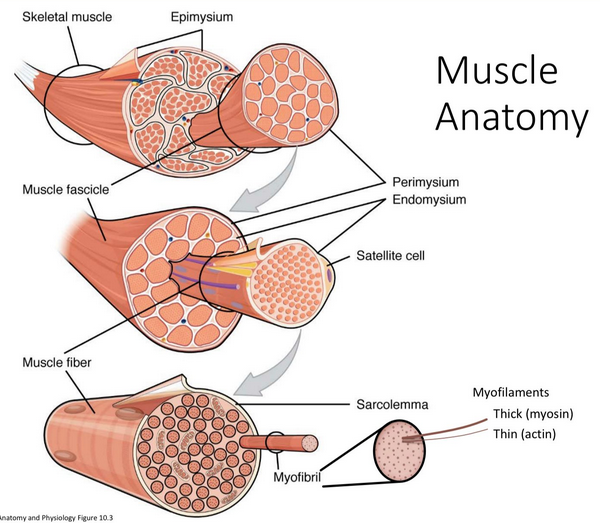
\includegraphics[width=0.6\textwidth]{muscleAnatomy}
            \caption{Muscle anatomy.}
            \label{fig:muscleAnatomy}
        \end{figure}
\end{itemize}

\subsection{Myofibrils}
\begin{itemize}
    \item myofibrils are the predominant structural feature of a skeletal muscle fibre (main working component of the muscle cell)
    \item made of myofilaments (thick is myosin, thin is actin)
\end{itemize}
\subsubsection{A and I Bands}
\begin{itemize}
    \item the A-band is Anisotropic, made up of a stacked set of thick filaments along with portions of thin filaments (produced by actin) that overlap on both ends of thick filaments (produced by myosin)
    \item the I-band consists of the remaining portion of the thin filaments that do not project into the A-band
    \item the H-zone is the lighter area (known as the "heller") within the middle of the A band where the thin filaments do not reach
    \item the M-line is known as the "middle line"
    \item the Z-line is in the middle of each I-band -- area between two Z-lines is called a \textbf{sacromere} 
    \item the stringy line things that holds myosin to the Z-line is a highly elastic protein called \textbf{titin} 
    \item muscle fibres function by having myofilaments sliding acros each other -- titin contracts and pulls thin filaments while thick filaments remain the same
    \item when muscles contract and relax, the H-zone and I-bands contracts and expands since titin is contracting/expanding
        \begin{itemize}
            \item the titin can be thought of as a spring that contracts and expands to move the muscle 
        \end{itemize}
    \item this movememnt causes the overall sacromere to expand or contract
        \begin{figure}[h]
            \centering
            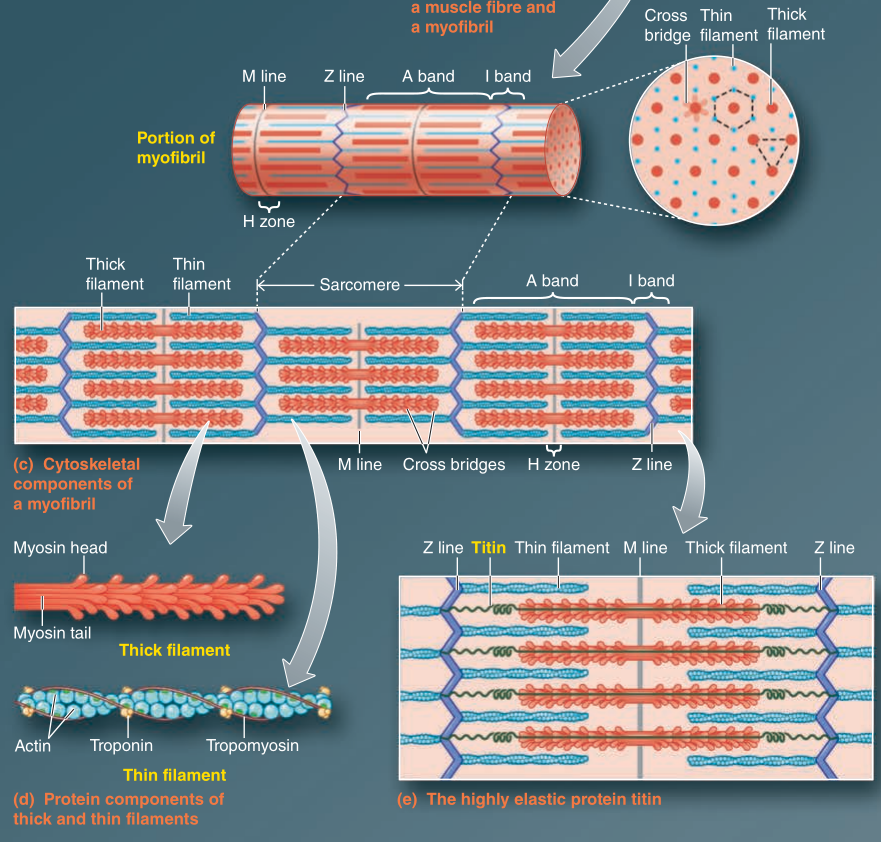
\includegraphics[width=0.8\textwidth]{myofibril}
            \caption{Myofibril.}
            \label{fig:myofibril}
        \end{figure}
\end{itemize}


\section{Skeletal Muscle Function (Excitation-Contraction Coupling)}
\begin{itemize}
    \item since nerves only interact with the outside of muscle fibres and there are many myofibrils inside a muscle fibre, how does the signal get to each myofibril?
    \item NMJ depolarizes the sarcolemma and then t-tubules allow electrical signal to travel down to myofibrils
    \item terminal cisternae (lateral sacs) are like reservoirs for calcium and are part of the sacroplasmic reticulum (SR)
        \begin{figure}[H]
            \centering
            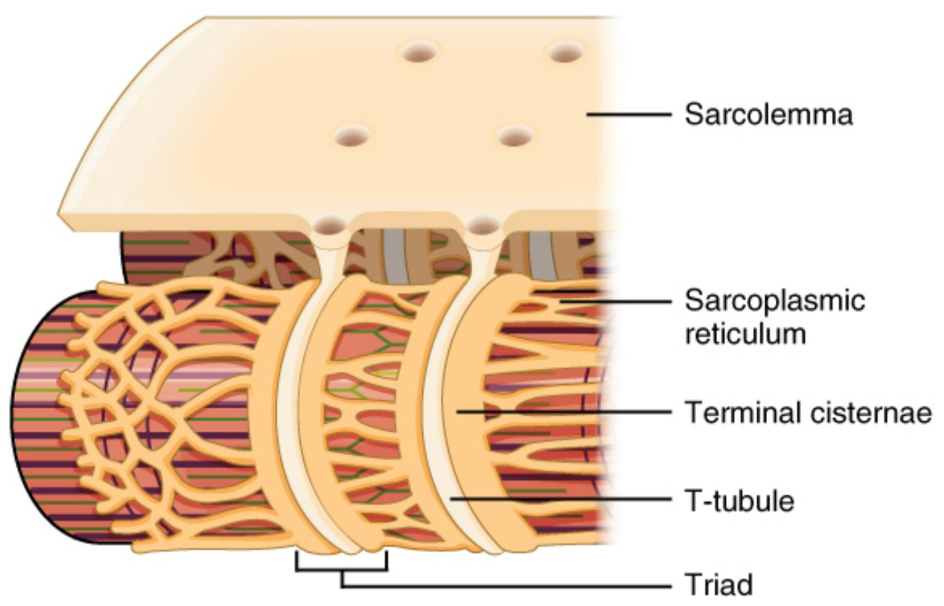
\includegraphics[width=0.8\textwidth]{lateralSacs}
            \caption{Terminal cisternae (lateral sacs).}
            \label{fig:lateralSacs}
        \end{figure}
        \begin{figure}[H]
            \centering
            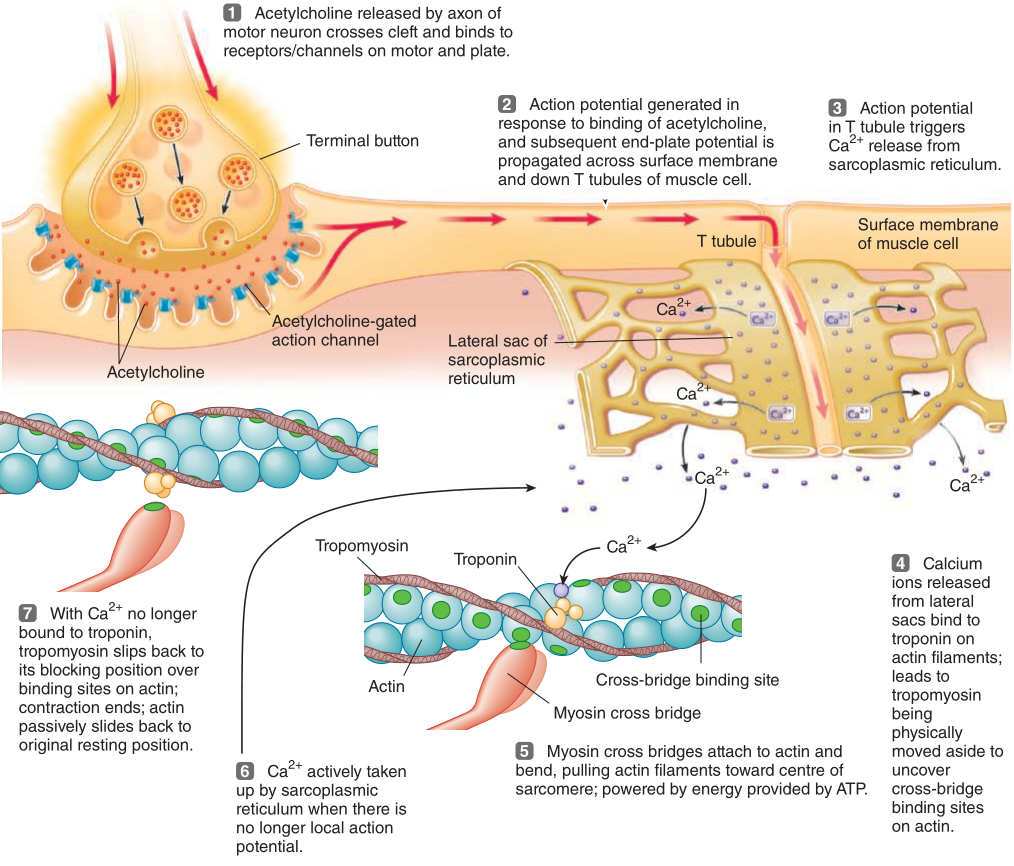
\includegraphics[width=0.8\textwidth]{molecularMuscleContraction}
            \caption{How muscles contract on a molecular level.}
            \label{fig:molecularMuscleContraction}
        \end{figure}
    \item neuron to muscle mapping is 1 neuron to 1 motor group (a few muscle cells)
    \item EPP travels down into t-tubules
    \item signal travels to sarcoplasmic reticulum (SR)
    \item allows calcium to be released into sarcoplasm
    \item calcium causes some stuff that leads to the whole muscle contracting
\end{itemize}

\subsection{Energy Supply to Skeletal Muscles -- Cross Bridge Cycling}
\begin{itemize}
    \item what happens when calcium is released into sarcoplasm -- how it causes muscle contraction
    \item the \textbf{cross-bridge link} is a secure structure that provides energy to muscle cells
\end{itemize}
\begin{enumerate}
    \item Energized stage: the myosin head brings ADP and inorganic phosphate but is bent slightly away from the thin filament
    \item Binding stage: the head bends to bind with the muscle fibre and forms the cross-bridge link
    \item Bending stage: the head bends even more (power stroke, applying 5 pN of force), releasing the phosphate first and ADP second
    \item Detachment stage: the head takes ATP formed by the released ADP and phosphate and detaches from the muscle fibre
        \begin{itemize}
            \item if no ATP, the myosin head is frozen on the thin filament
        \end{itemize}
    \item Reattachment: ATP is broken down into ADP and phosphate (hydrolyzed/dephosphorylated)
\end{enumerate}
\begin{itemize}
    \item note that in the case of no ATP, the muscle cell is frozen -- \textbf{rigor mortis} 
    \item calcium moves the troponin complex out of the way
    \item pulls the tropomyosin latch open
    \item exposes all the cross-bridge binding sites located on the actin (thin filament)
    \item to relax, the reverse steps happen
\end{itemize}


\section{Skeletal Muscle Mechanics}
\begin{itemize}
    \item rebar is to concrete as muscle is to bone (functionally)
    \item types of contractions:
        \begin{itemize}
            \item concentric -- muscle contracts
            \item eccentric -- muscle elongates
            \item isometric -- muscle contracts but stays in place
        \end{itemize}
\end{itemize}

\subsection{Tension Developed by Each Fibre}
\subsubsection{Action Potential Frequency}
\begin{figure}[H]
    \centering
    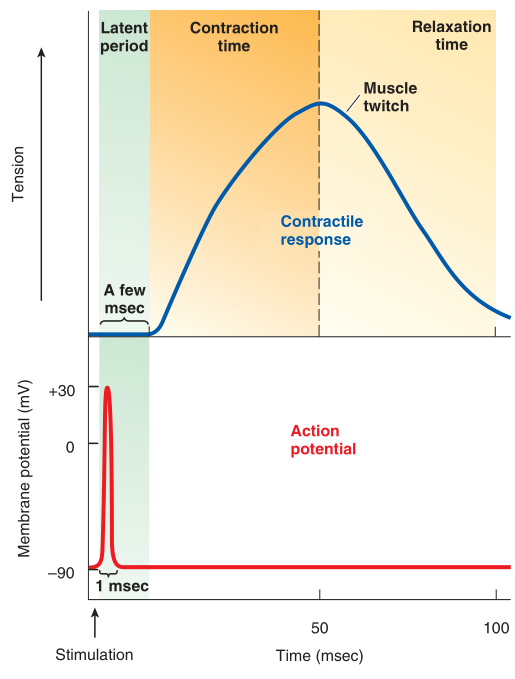
\includegraphics[width=0.8\textwidth]{muscleActionPotential}
    \caption{Relationship between action potential and resultant muscle twitch.}
    \label{fig:muscleActionPotential}
\end{figure}
\begin{figure}[H]
    \centering
    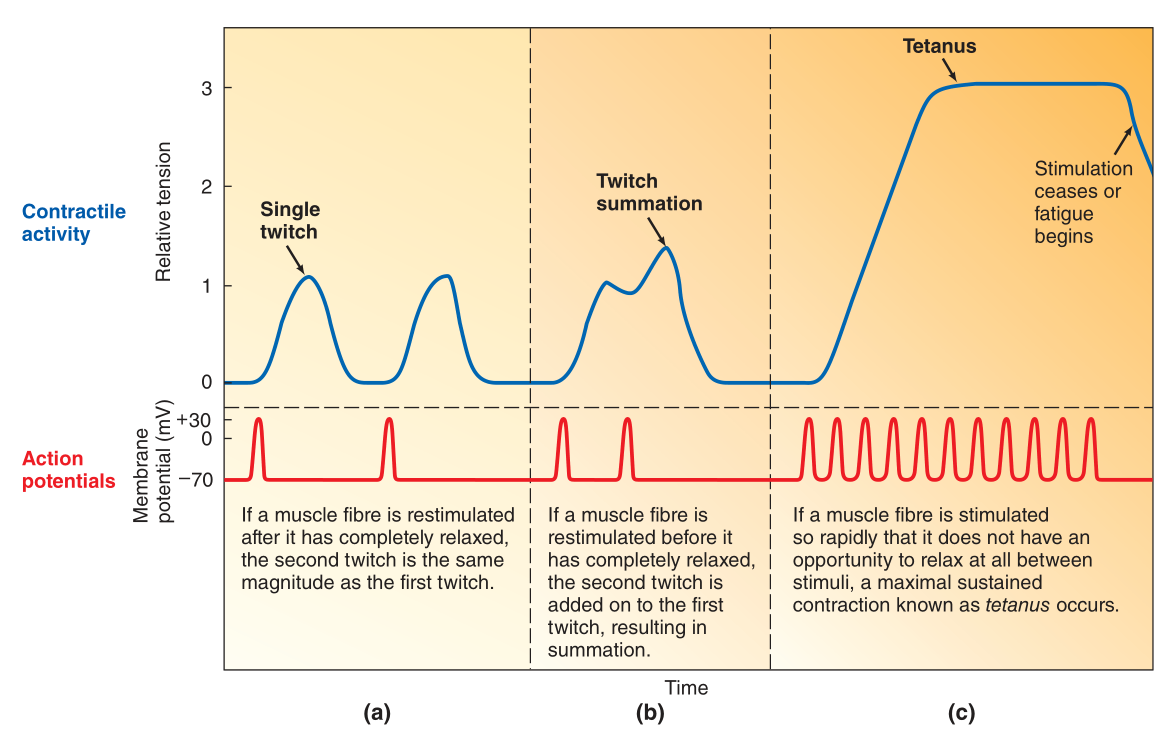
\includegraphics[width=0.8\textwidth]{summationTetanus}
    \caption{Summation and tetanus.}
    \label{fig:summationTetanus}
\end{figure}
\begin{itemize}
    \item after a high enough stimulation frequency, it causes twitch summation and there is a tetanic maximum that a muscle can contract to
    \item around 100 Hz is what causes tetanus
\end{itemize}

\subsubsection{Fibre Length}
\begin{figure}[H]
    \centering
    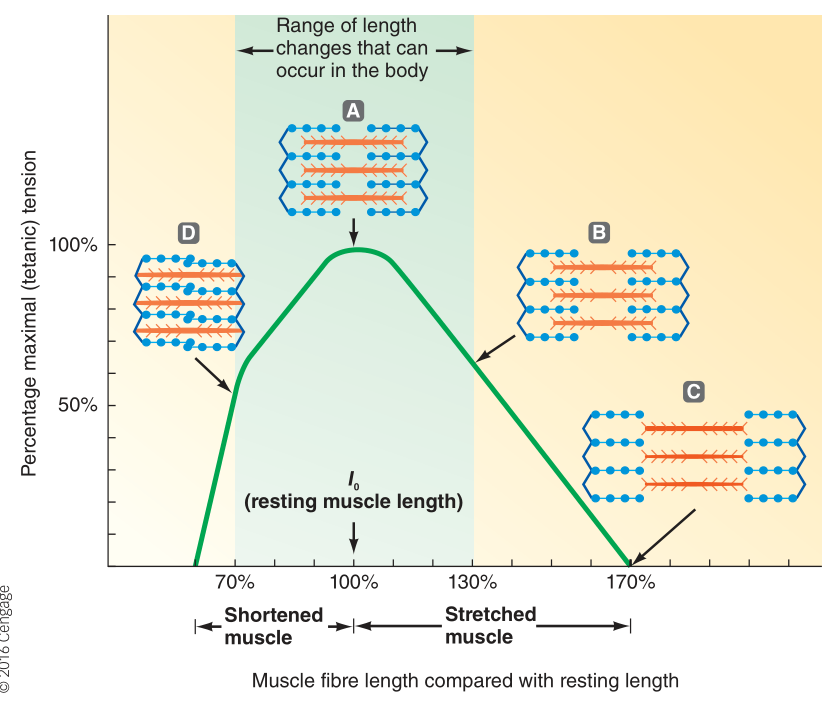
\includegraphics[width=0.8\textwidth]{muscleLengthTension}
    \caption{Length-tension relationship.}
    \label{fig:muscleLengthTension}
\end{figure}
\begin{itemize}
    \item there is also some passive length-tension due to titin being stretched or compressed
\end{itemize}

\subsubsection{Fibre Diameter}
\begin{itemize}
    \item fibre hypertrophy -- bigger myofibrils (swole) caused by growing bigger Z disc
    \item fibre splitting or hyperplasia -- more myofibrils (ripped) caused by tearing Z disc
    \item smaller diameter = less force, larger diameter = more force
\end{itemize}

\subsubsection{Fatigue}
\begin{itemize}
    \item type 1 fibres don't fatigue very much (can sustain tension for long time)
    \item type 2A fatigues quickly
    \item type 2X fatigue very quickly
    \item factors that influence muscle fatigue:
        \begin{itemize}
            \item ADP interferes with cross-bridge
            \item Accumulation of lactic acid (interferes with making more ATP)
            \item increased extracellular K (stops depolarization)
            \item depletion of glycogen energy reserves
        \end{itemize}
\end{itemize}

\subsubsection{Fibre Type}
\begin{itemize}
    \item mitochondria: many in slow twich (type 1), less in fast twitch (type 2)
    \item capillaries: many in slow and type 2A, few in type 2X
    \item myoglobin content: high in slow and 2A, low in 2X
    \item contraction velocity: slow in slow, fast in 2A, fastest in 2X
    \item size of motor neuron innervating fibre: smaller in slow, larger in fast, largest in type 2X
\end{itemize}


\subsection{Number of Active Fibres}
\subsubsection{Number of fibres per motor unit}
\begin{itemize}
    \item more muscle fibres recruited = more power
\end{itemize}

\subsubsection{Number of active motor units}
\begin{itemize}
    \item different motor neurons control different motor units (slow twitch, fast twitch)
\end{itemize}





\section{Smooth Muscles}
\begin{itemize}
    \item smooth muscles are found in STOVE:
        \begin{itemize}
            \item Skin
            \item Tracts (such as gastrointestinal tract)
            \item Hollow Organs (e.g. stomach)
            \item Vessels
            \item Eyes
        \end{itemize}
\end{itemize}

\subsection{Structure of Smooth Muscles}
\begin{itemize}
    \item in the relaxed state:
        \begin{figure}[H]
            \centering
            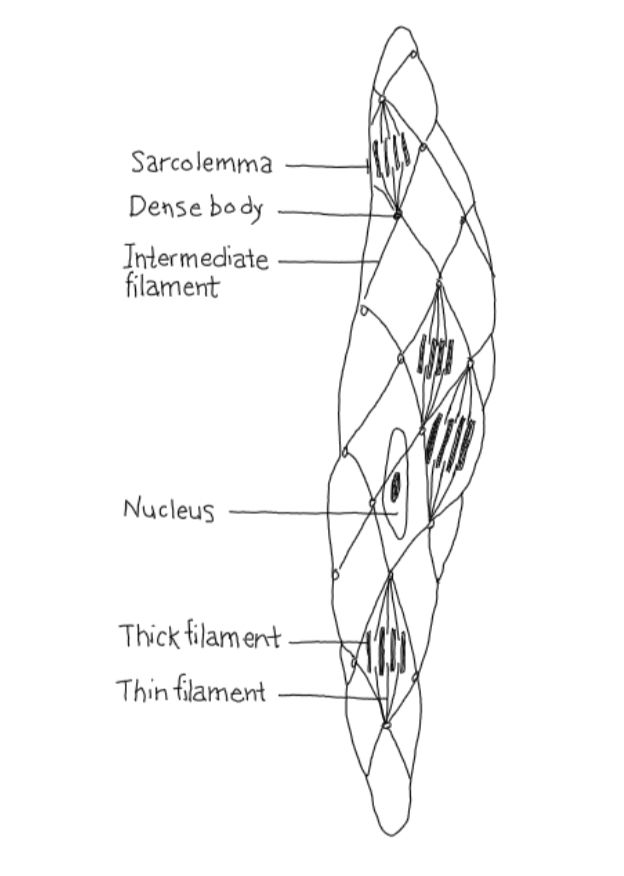
\includegraphics[width=0.3\textwidth]{smoothMuscleRelaxed.jpeg}
            \caption{Relaxed smooth muscle.}
            \label{fig:smoothMuscleRelaxed}
        \end{figure}
    \item in the contracted state: 
        \begin{figure}[H]
            \centering
            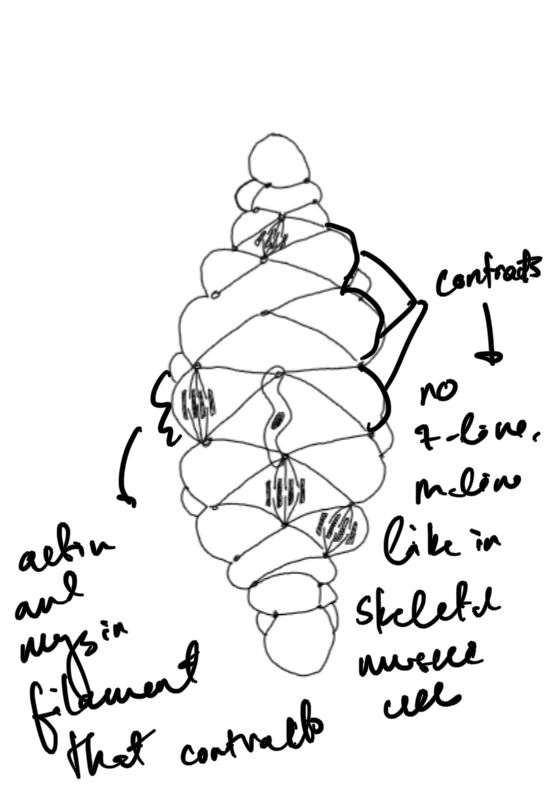
\includegraphics[width=0.5\textwidth]{smoothMuscleContracted.jpeg}
            \caption{Contracted smooth muscle.}
            \label{fig:smoothMuscleContracted}
        \end{figure}
    \item these are innervated by the autonomic nervous system 
    \item they can be initiated either by neurogenic or myogenic causes
    \item nervous stimulation can modify contraction, excite or inhibit, and contribute to gradation
    \item gradation is accomplished mainly via varying number of muscle fibres, varying cystolic Ca$^2+$, as well as autonomic, hormonal, mechanical stretch, and metabolites
    \item these are affected by hormones and have poorly developed sarcoplasmic reticulum
    \item they also have gap junctions
    \item main source of Ca is ECF
\end{itemize}

\subsection{Types of Smooth Muscle}
\begin{itemize}
    \item Single-unit and multi-unit smooth muscles 
    \item multi-unit muscles consist of multiple discrete units that function independently of one another 
        \begin{itemize}
            \item separately stimulated by nerves to contract (similar to skeletal muscle) -- neurogenic
            \item multi-unit muscles do not have gap junctions between the muscle cells and have more motor neurons to control precisely how each fibre contracts and expands
        \end{itemize}
    \item single unit muscles contract as a single unit
        \begin{itemize}
            \item single unit muscle fibres are electrically linked by gap junctions
        \end{itemize}
        \begin{figure}[h]
            \centering
            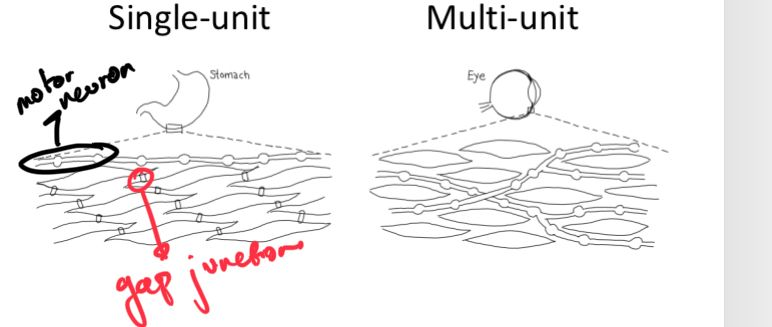
\includegraphics[width=0.8\textwidth]{singleMultiUnitSmoothMuscles.jpeg}
            \caption{Single and multiunit smooth muscles.}
            \label{fig:singleMultiUnitSmoothMuscles}
        \end{figure}
\end{itemize}









\part{Cardiac Physiology}
\section{Cardiac Muscle}
\begin{itemize}
    \item cardiac muscle is wrapped in curvy circular ways
    \item there is significant variation in the type of cardiac muscles depending on where they are 
    \item both skeletal and cardiac muscles are \textbf{striated} (has alternating dark and light bands -- repeating sacromeres)
        \begin{itemize}
            \item they have the actin and myoactin mechanisms for function with the push and pull mechanism for motion
            \item cardiac muscle is involuntary, skeletal muscle is voluntary
        \end{itemize}
    \item calcium plays a role in depolarization in the heart
\end{itemize}
\begin{table} % use table to add captions
    \begin{center}
        \caption{Differences between skeletal and cardiac muscle.}
        \begin{tabular}{|p{7cm}|p{7cm}|} 
             \hline\hline
             \textbf{Skeletal Muscle}  & \textbf{Cardiac Muscle}  \\
             \hline
             Innervated using the somatic nervous system & Innervated using the autonomic nervous system \\
             \hline
             Initiated due to neurogenic causes & Initiated due to myogenic causes -- initiated by muscle cells \\
             \hline
             Initiates contraction and achieves gradation & Modifies contraction through excitement and inhibition \\
             \hline
             Gradation accomplished by number of motor units, frequency summation & Gradation by varying length of muscle fibres and Ca$^2+$ amount in cytosol \\ 
             \hline
             Not affected by hormones & Affected by hormones \\ 
             \hline
             Well developed sarcoplasmic reticulum & Moderately developed sarcoplasmic reticulum (mainly gets Ca from ECF)\\ 
             \hline 
             No gap junctions & Has gap junctions \\ 
             \hline\hline
        \end{tabular}
        \label{skeletalVsCardiacMuscle}
    \end{center}
\end{table}


\section{Electrical Activity of the Heart}
\begin{itemize}
    \item cardiac muscle has a much higher concentration of mitochondria -- needs to constantly open and close ion channels to keep heart beating
    \item electrical activity starts in right atrium, travels in this order: sinoatrial node, atrial muscle, atrioventricular node, Purkinje fibres, ventricular muscle
    \item in a skeletal muscle fibre, Na$^+$ comes into the cell upon initiation of an action potential with a delayed inflow of K$^+$ due to the slow initiation for the voltage gated channels 
    \item in the heart, different types of muscles have different polarization patterns
        \begin{itemize}
            \item these patterns spread due to the gap junctions between cardiac fibres
        \end{itemize}
    \begin{figure}[H]
        \centering
        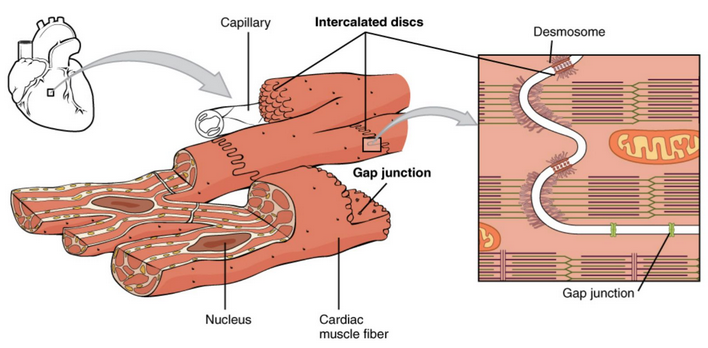
\includegraphics[width=0.8\textwidth]{cardiacGapJunctions}
        \caption{Gap junctions between cardiac fibres.}
        \label{fig:cardiacGapJunctions}
    \end{figure}
    \begin{figure}[H]
        \centering
        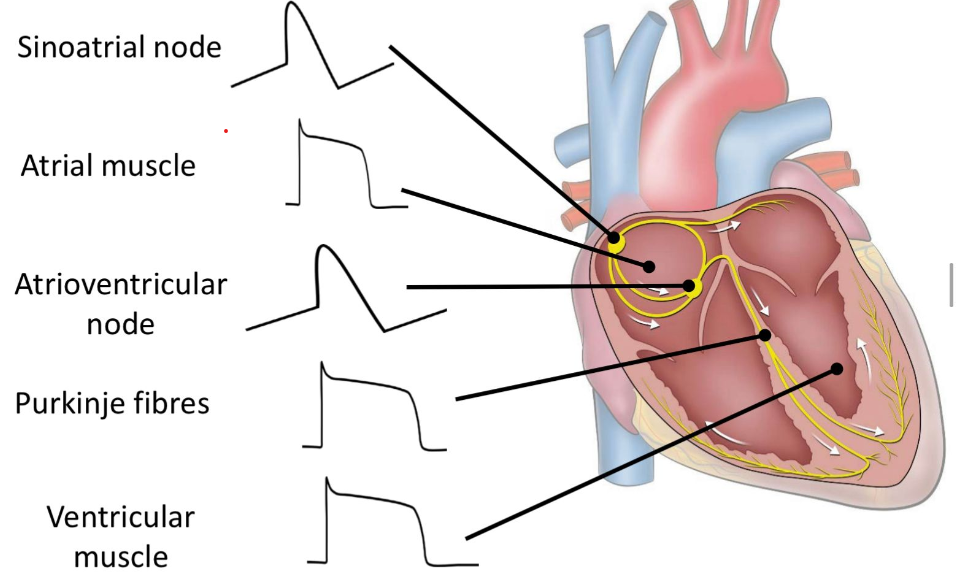
\includegraphics[width=0.8\textwidth]{cardiacMusclePolarizationPatterns}
        \caption{Different polarization patterns for different types of muscles in the heart.}
        \label{fig:cardiacMusclePolarizationPatterns}
    \end{figure}
\end{itemize}

\subsection{Ventricular Myocyte Action Potential}
\begin{figure}[H]
    \centering
    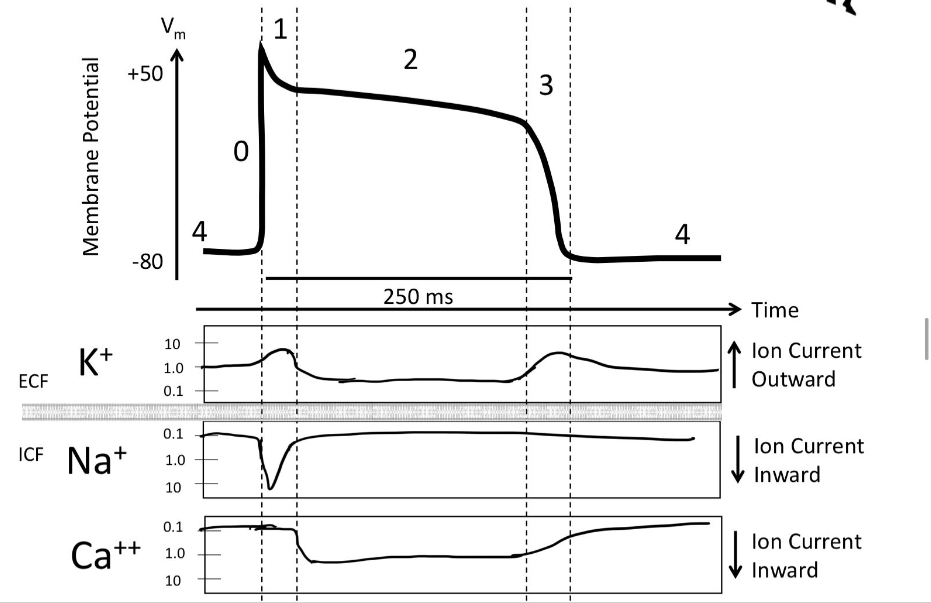
\includegraphics[width=0.8\textwidth]{ventricularExcitation}
    \caption{Action potential in ventricular muscle cells.}
    \label{fig:ventricularExcitation}
\end{figure}
\begin{itemize}
    \item Phase 4 -- normal resting state (resting membrane potential)
    \item Phase 0 -- rapid depolarization which while not instantaneous, is very very quick
    \item Phase 1 is caused due to K channels which cause a slight depolarization
    \item Phase 2 -- K$^+$ going out while Ca$^{2+}$ going in causes a plateau
    \item Phase 3 -- more K$^+$ channels open, which expel these ions, causing a rapid depolarization
\end{itemize}
\begin{figure}[H]
    \centering
    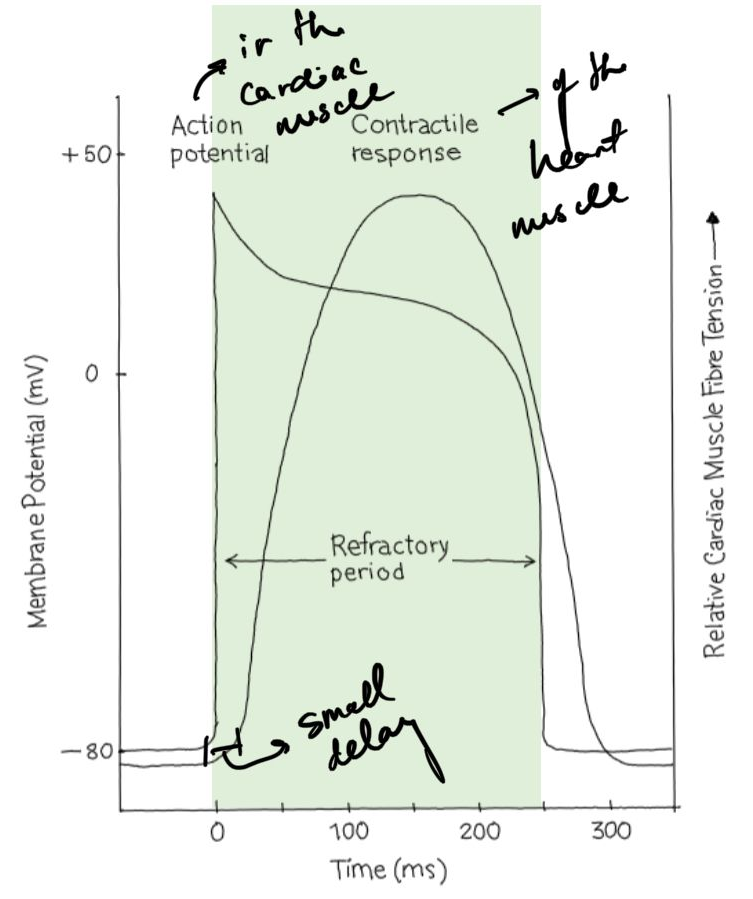
\includegraphics[width=0.8\textwidth]{cardiacMuscleContractileResponse}
    \caption{Relationship of an action potential and the refractory period to the duration of the contractile response in cardiac muscle.}
    \label{fig:cardiacMuscleContractileResponse}
\end{figure}
\begin{itemize}
    \item the refractory phase prevents frequency summation and allows the muscle to relax
        \begin{itemize}
            \item without this the muscle would not be able to expel or take in blood
        \end{itemize}
\end{itemize}

\subsection{Pacemaker (Nodal) Cells}
\begin{figure}[h]
    \centering
    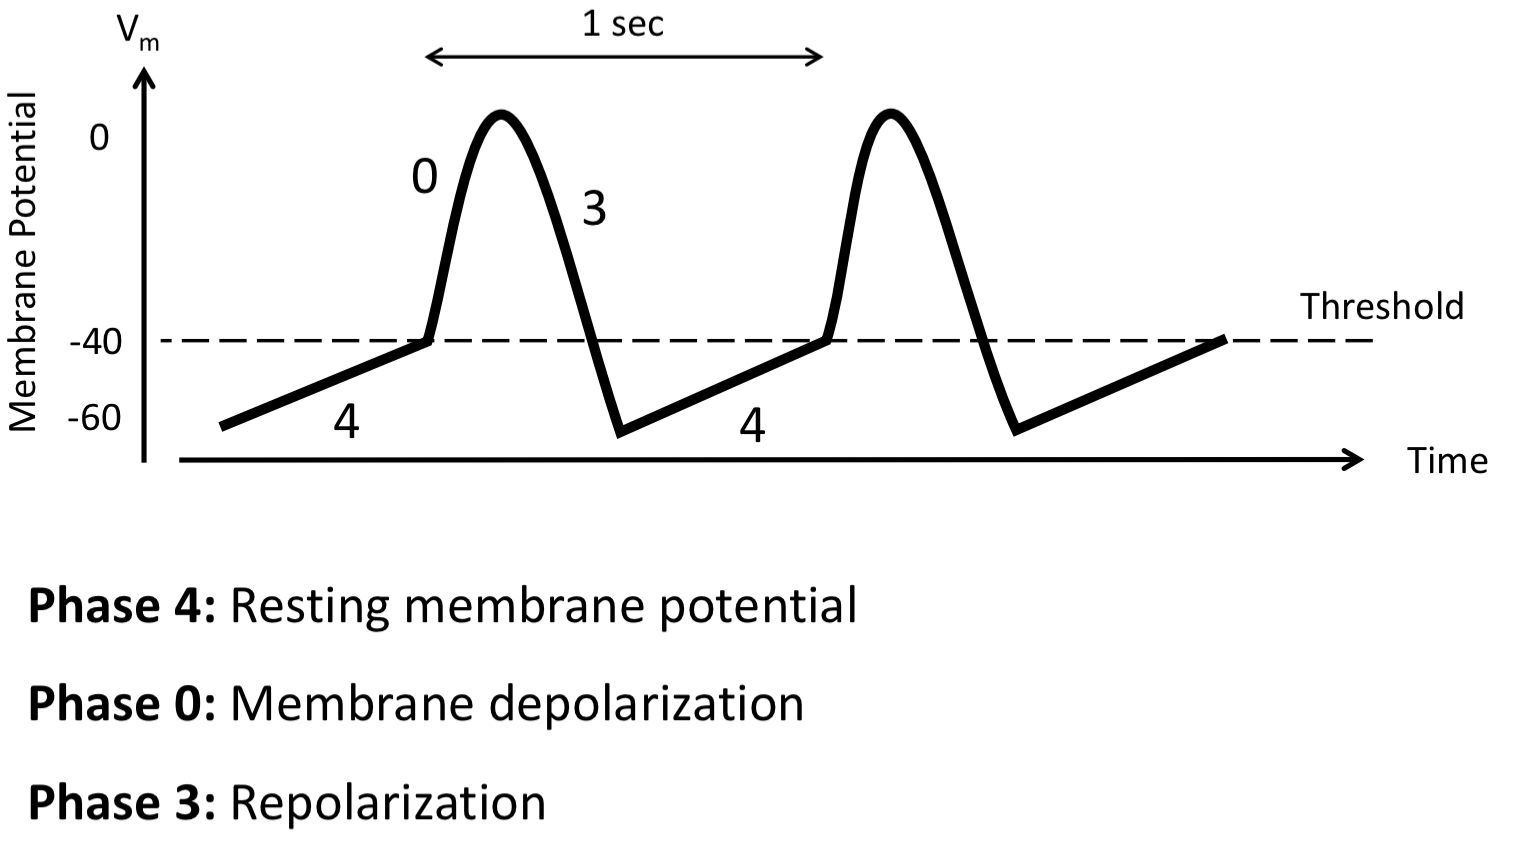
\includegraphics[width=0.8\textwidth]{pacemakerActionPotential.jpeg}
    \caption{Pacemaker activity of cardiac autorhythmic cells.}
    \label{fig:pacemakerActionPotential.jpeg}
\end{figure}
\begin{figure}[h]
    \centering
    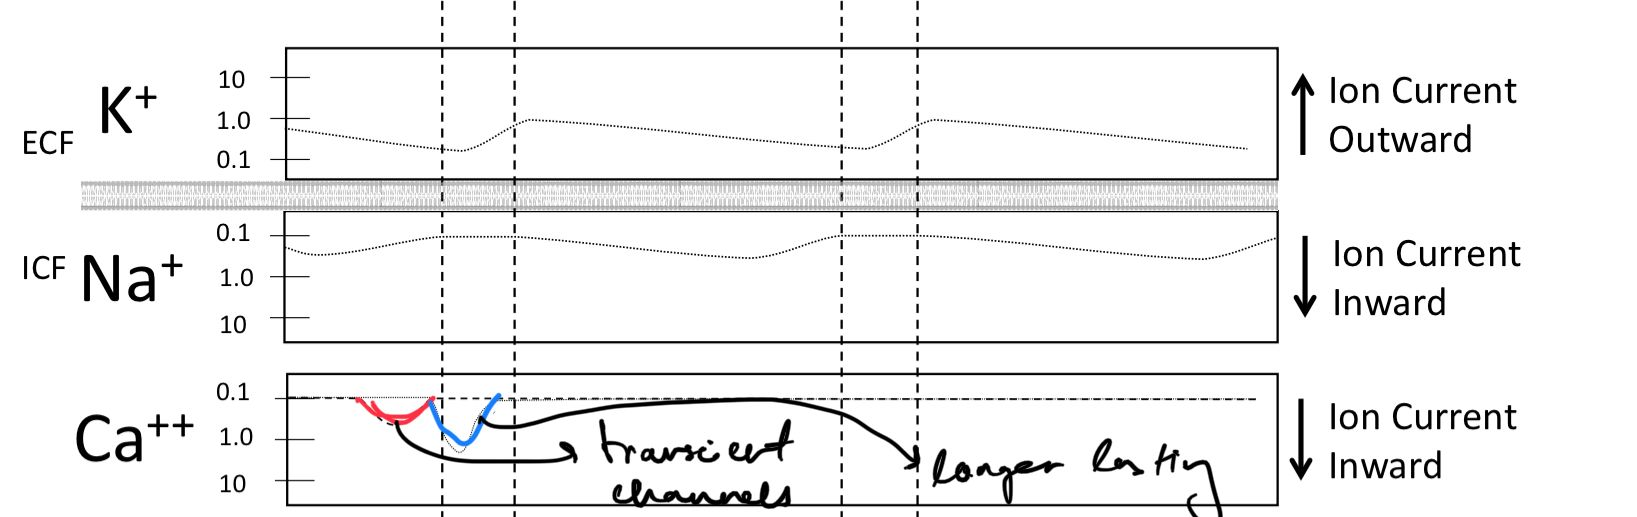
\includegraphics[width=0.8\textwidth]{pacemakerIonConcentration.jpeg}
    \caption{Ion concentrations during pacemaker activity.}
    \label{fig:pacemakerIonConcentration.jpeg}
\end{figure}
\begin{itemize}
    \item Calcium causes the depolarization (instead of the sodium in ventricular muscles)
    \item transient channels are known as \textbf{T channels} while longer lasting channels are known as \textbf{L channels} 
    \item heartrate modulation:
        \begin{itemize}
            \item rate of depolarization: decreased rate causes a lower heart rate (takes longer to reach threshold) 
            \item more hyperpolarized: requires more time to reach threshold (decreases heart rate)
            \item shift in threshold: a lower threshold causes a longer time to depolarize and hence a lower heart rate; higher threshold causes higher heart rate
        \end{itemize}
\end{itemize}

\subsection{Electrocardiogram (ECG)}
\begin{itemize}
    \item positive deflection on ECG can be depolarization moving toward electrode or repolarization moving away from electrode
    \item direction of electrical activity: 
        \begin{itemize}
            \item depolarize atria (P wave): sinoatrial node, atrial pathways, atrioventricular node
            \item depolarize septum from left to right (Q, R, and S wave): atrioventricular node, Bundle of His, Purkinje system (faster conduction velocity)
            \item depolarize ventricular muscle: Purkinje system, ventricular muscle, endocardium, epicardium
            \item repolarization occurs in reverse order (ventricular first) (T wave)
        \end{itemize}
    \item physical trauma to the heart during the T wave may cause ventricular fibrilation -- could trigger another depolarization
\end{itemize}

\subsubsection{Matching ECG to Pumping Actions}
\begin{itemize}
    \item major events of cardiac cycle:
        \begin{itemize}
            \item ventricular diastole
                \begin{itemize}
                    \item passive filling
                    \item atrial ejection
                \end{itemize}
            \item ventricular systole
                \begin{itemize}
                    \item isovolumic ventricular contraction
                    \item ventricular ejection
                \end{itemize}
            \item ventricular diastole 
                \begin{itemize}
                    \item isovolumic ventricular relaxation
                \end{itemize}
        \end{itemize}
\end{itemize}
\begin{figure}[H]
    \centering
    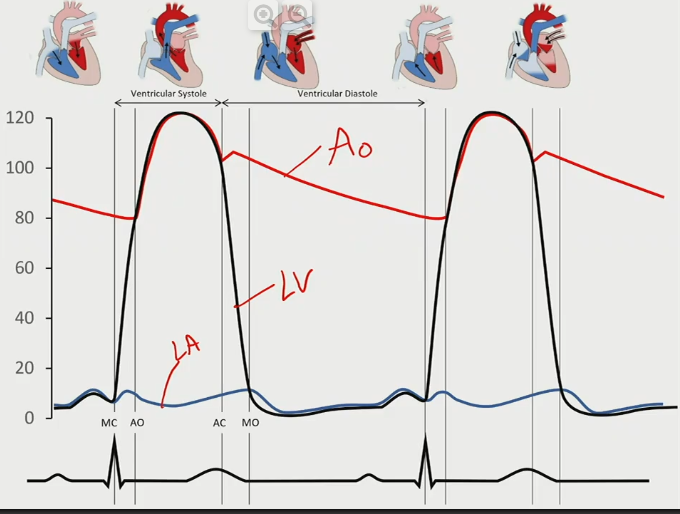
\includegraphics[width=0.8\textwidth]{ECGToPump}
    \caption{Matching ECG to pumping actions.}
    \label{fig:ECGToPump}
\end{figure}

\subsubsection{Volume of Blood Inside Heart}
\begin{itemize}
    \item left ventricular stroke volume (typically around 70mL) is given by:
        \begin{gather*}
            SV = EDV - ESV
        .\end{gather*}
    \item where EDV is end diastolic volume (135 mL), ESV is end systolic volume (65 mL)
\end{itemize}



\section{Cardiac Regulation}
\begin{itemize}
    \item cardiac output (L/min) is given by the product of stroke volume and heart rate:
        \begin{gather*}
            CO = SV \cdot HR
        .\end{gather*}
    \item SV and HR are the two main factors that influence cardiac output
\end{itemize}

\subsection{Heart Rate}
\begin{itemize}
    \item autonomic effects on the heart
        \begin{itemize}
            \item cardiovascular center in the medulla sends signals to heart
            \item vagus nerve triggers atrial muscle (parasympathetic stimulation)
                \begin{itemize}
                    \item the vagus nerve releases ACh that increases the permeability of the SA node to K by slowing the clsure of K voltage-gated channels
                    \item this lowers the minimum diastolic potential -- depolarization takes longer to reach back to threshold
                    \item also decreases the rate of depolarization -- enhanced K permeability opposes the pacemaker current (resulting from Na and K currents) responsible for the gradual depolarization
                \end{itemize}
            \item sympathetic nerves trigger ventricular myocytes
                \begin{itemize}
                    \item sympathetic nerves releases norepinephrine (NE) that binds to the $\beta 1$ adrenergic receptors, that functionally increase the HR
                    \item increases the pacemaker current -- increases rate of depolarization and reaches threshold faster
                    \item increases Ca currents makes Ca voltage-gated channels more active and threshold potential is lowered -- takes less time to reach threshold
                    \item greater sympathetic stimulation increases calcium permeability which increases conduction velocity for the AV node and Purkinje fibres
                \end{itemize}
            \item need vagal and sympathetic tone (how much ACh or NE is dripping out from the nerves) to decrease/increase your heart rate
        \end{itemize}
\end{itemize}

\subsection{Stroke Volume}
\subsubsection{Intrinsic Control of SV}
\begin{theorem}
    \textbf{Frank-Starling Law}: the more you stretch the heart muscle, the more force it develops
\end{theorem}
\subsubsection{Extrinsic Control of SV}
\begin{itemize}
    \item sympathetic nerves are the only ones that go to the ventricular muscles
    \item increased Ca permeability increases Ca currents and availability in cytosol of ventricular myocytes
    \item this increases the force developed by ventricular myocytes and force of ventricular contraction
    \item ultimately increases SV
\end{itemize}













\part{Vascular Physiology}






















\end{document}

